\documentclass{beamer}
\usetheme{afm}

\title{Interest Rate Derivatives}
\subtitle{Main Ineterst Rate Contracts Theory}
\course{Advanced Financial Modelling}
\author{\href{mailto:matteo.sani@unisi.it}{Matteo Sani}}

\begin{document}
\begin{frame}[plain]
  \maketitle
\end{frame}

\begin{frame}{Single Curve Approach}
	\begin{block}{Disclaimer}
	What follows is a detailed exposition of the classic \textcolor{red}{single curve}
	approach for interest rate derivatives. 
	
	Today a \textcolor{red}{multi-curve approach} is
	used in practical applications. Nevertheless you need to understand
	deeply this basic approach as a prerequisite for the extension to the
	multi-curve model.
	\end{block}
\end{frame}  

\subsection{Money Market Account}
\begin{frame}{Money Market Account}
	\begin{itemize}
		\item<0-> The \textcolor{red}{money market account} represents a risk-less investment, where profit is accrued continuously at the risk-free rate, and its value is denoted by $B(t)$.
		\item<1-> We assume $B(0)=1$ and by definition
		\begin{equation}
			dB(t) = r(t)B(t)dt
		\end{equation}
		\item<2-> This evolution can be solved through variable separation
		\begin{equation}
			\begin{gathered}
				\frac{dB_t}{B_t} = r_t dt \implies \int_0^t \frac{dB_t}{B_t} = \int_0^t r_s ds \\
				\implies \log\frac{B_t}{B_0} = \int_0^t r_s ds \implies \boxed{B(t) = \exp\left(\int_0^t r_s ds\right)}
			\end{gathered}
		\end{equation}
		where $r_t$ is referred to as \textcolor{red}{instantaneous spot rate} or \textcolor{red}{short rate}.
	\end{itemize}
\end{frame}

\begin{frame}{Money Market Account}
	\begin{itemize}
		\item<0-> The \emph{short rate} $r_t$ can be modeled either by a deterministic or a stochastic process.
		\item<1-> \textbf{Deterministic case}: from the definition of money market account it follows that 
		\begin{equation*}
			V(0) = A \implies V(t) = A\cdot B(t)
		\end{equation*}
		\item<2-> If we want to have at time $T$ exactly 1 unit of currency
		\begin{equation*}
			AB(T) = 1 \implies AB(t) = \frac{B(t)}{B(T)} 
		\end{equation*}
		hence $\frac{B(t)}{B(T)}$ is \textcolor{red}{the value of one unit of currency payable at time $T$ seen from $t$}.
		
		%%		\item We now define the abstract quantity $r(t)$, the \textbf{short rate}, as
		%%		\begin{equation}
			%%			r(t) = \lim_{T\rightarrow t^+} L(t,T) \simeq L(t, t+\epsilon)
			%%		\end{equation}\quad with $\epsilon$ small
	\end{itemize}
\end{frame}

\subsection{Stochastic Discount Factor and Zero Coupon Bond}
\begin{frame}{Stochastic Discount Factor}
	\uncover<1->{
		\begin{block}{Defintion}
			The \textcolor{red}{(stochastic) discount factor} $D(t, T)$ is the amount at time $t$ that is \emph{equivalent} to one unit of currency payable at time $T$ and is given by
			\begin{equation}
				D(t, T) = \frac{B(t)}{B(T)} = e^{-\int_t^T r_s ds}
			\end{equation}
	\end{block}}
	\begin{itemize}
		\item<2-> Can you guess which are its dimensions ?	
		\item<3-> In many pricing application (e.g. Black-Scholes formula) $r$ is assumed to be a \textcolor{red}{deterministic} function of time, and so are $B(t)$ and $D(t,T)$:
		\begin{itemize}
			\item<3-> this is motivated by the small influence interest rate variations have on equity prices.
		\end{itemize}
		\item<4-> When dealing with interest rate products, $r$ becomes the main actor, so the deterministic assumption must be dropped.
	\end{itemize}	
\end{frame}

\begin{frame}{Deterministic vs Stochastic}
	\begin{itemize}
		\item<0-> Recall the risk-neutral pricing formula \begin{equation*}
			\Pi_t = \expect{Q^B}[D(t,T)A|\mathcal{F}_t]
		\end{equation*}
		where the corresponding risk-neutral measure is often denoted by $\mathbb{Q}^0$ or $\mathbb{Q}^B$, and similarly for the expectations. 
		%	In the following we are going to use $B(t)$ as numeraire then  Eq.~\ref{eq:risk_neutral_pricing} becomes
		%	\begin{equation*}
			%		\begin{aligned}
				%			S_t = \mathbb{E}^{\mathcal{Q}^B}\left[e^{-\int_t^T r_s ds}S_T|\mathcal{F}_t\right]
				%		\end{aligned}
			%	\end{equation*}
		%	where $\mathcal{Q}^B$ is the risk-neutral measure.% that makes $\frac{S_t}{B_t}$ a martingale. 	
		\item<1-> When \textcolor{red}{interest rates are deterministic}, the exponential can be brought out of the expectation
		\begin{equation*}
			\Pi_t = e^{-\int_t^T r_s ds} \expect{B}\left[A|\mathcal{F}_t\right]
		\end{equation*}
		\item<2-> Instead when \textcolor{red}{rates are constant} (e.g. Black-Scholes or Heston models)
		\begin{equation*}
			\Pi_t = e^{-r(T-t)}\expect{B}\left[A|\mathcal{F}_t\right]
		\end{equation*}
	\end{itemize}
\end{frame}

\begin{frame}{Zero Coupon Bond}
	\begin{itemize}
		\item<0-> \textcolor{red}{Zero Coupon Bond} (ZCB) is a contract that pays one unit of money at time $T$. Its price at time $t$ is denoted by $P(t,T)$, and by definition $P(T,T) = 1$.
		\item<0-> What is the relation between $P(t,T)$ and $D(t,T)$ ? \\
		\uncover<1->{
			\renewcommand{\arraystretch}{1.2}
			{\tiny {\tiny }}{
				\begin{table}[bt]
					\begin{tabular}{|c|c|} \hline
						$D(t, T)$ & $P(t, T)$ \\ \hline
						equivalent amount of money & value of a contract \\ \hline
						\multicolumn{2}{|c|}{\textcolor{red}{deterministic rates}} \\ \hline
						\multicolumn{2}{|c|}{D(t,T)=P(t,T)} \\ \hline 
						\multicolumn{2}{|c|}{\textcolor{red}{stochastic rates}} \\ \hline
						random quantity at time $t$ &
						\renewcommand{\arraystretch}{1.0} 
						\begin{tabular}{@{}c@{}}
							being the value of a contract\\ with a payoff at time $T$, must be known in $t$ \\
							from 
							$P(t, T) = \expect{Q}[D(t, T)|\mathcal{F}_t]$
						\end{tabular} \\ \hline
					\end{tabular}
				\end{table}
		}}
	\end{itemize}
\end{frame}

%\begin{frame}{Year Fraction, Day-Count Convention}
%	\begin{itemize}
%		\item Time to maturity: $T-t$
%		\item Denote by $\tau(t, T)$ the chosen time measure between $t$ and $T$. In theory, you can think of $\tau(t, T)=T-t$. In practice there are many possible ways to compute that time difference.
%		\item Among the plethora of conventions, the followings are worth mentioning:
%		\begin{itemize}
%			\item Actual/365
%			\item Actual/360
%			\item 30/360
%		\end{itemize}
%		\item \textcolor{red}{Go and find their definitions: they are also embedded in Excel as financial functions.}
%	\end{itemize}
%	\begin{tikzpicture}[remember picture,overlay]
%		\node[xshift=5cm,yshift=-3.7cm] (image) at (current page.center) {
\includegraphics[width=20px]{python_logo}};
%		\node[align = center, yshift=1.45cm, below=of image] {\tiny{\href{shorturl.at/chzT2}{shorturl.at/chzT2}}};
%	\end{tikzpicture}
%\end{frame}

\subsection{Spot Interest Rate}
\begin{frame}{Spot Interest Rate}
	\begin{itemize}
		\item Simply-compounded \textcolor{red}{spot interest rate}
		\begin{equation}
			L(t,T)=\frac{(1-P(t,T))}{\tau(t,T)P(t,T)}		
		\end{equation}
		\item The \textcolor{red}{yield curve} at time $t$ is the graph of:
		\begin{equation*}
			T\rightarrowtail L(t, T)
		\end{equation*}
		\item In the market these are the so called LIBOR (or EURIBOR) rates and are typically compounded with the actual/360 convention. They are the main rates underlying interest rate derivatives.
	\end{itemize}
\end{frame}

\section{Forward Rate Agreement}
\begin{frame}{Forward Rate Agreement}
	\begin{itemize}	
		\item<1-> A \textcolor{red}{Forward Rate Agreement} (FRA) is a contract involving three time instants: %the current time $t$, the fixing time $T>t$, and the maturity time $S>T$.
		\begin{equation*}
			\underbrace{t}_{\text{current time}} \leq \underbrace{T}_{\text{fixing time}} \leq\underbrace{S}_{\text{maturity}}
		\end{equation*}
		\item<2-> The FRA payout consists of an exchange of interest rate flows calculated for the time period $\tau=S-T$. At the maturity $S$, a fixed payment based on a fixed rate $K$ is exchanged against a floating payment based on the spot rate $L(T, S)$ whose value is known only in $T$.
		\item<3-> Basically, this contract allows one to lock-in the interest rate between times $T$ and $S$ at a desired value $K$.
		 
		\noindent
		(\textbf{note:} interest rate flows are calculated using the simple compounding law).
	\end{itemize}
\end{frame}

\begin{frame}{Forward Rate Agreement}
	\begin{itemize}
	\item A FRA is an agreement that enables to \emph{hedge} against unfavourable movements in interest rates by fixing a rate on a notional amount that is (usually) of the same size and term as the exposure that starts sometime in the future. 
	\vfill
	\begin{center}
		\includegraphics[width=0.9\linewidth]{FRA_diagram}
	\end{center}
	\end{itemize}
\end{frame}

\begin{frame}{FRA Example}
	\begin{itemize}
		\item Consider a $1\times 3$ FRA (1-month into 3-month): the 1 in the $1\times 3$ refers to 1 month' time when settlement (fixing) takes place, and the 3 to the expiry date of the FRA from deal date, i.e. the rate quoted for the FRA is a 1-month rate at the time of settlement
	\begin{center}
		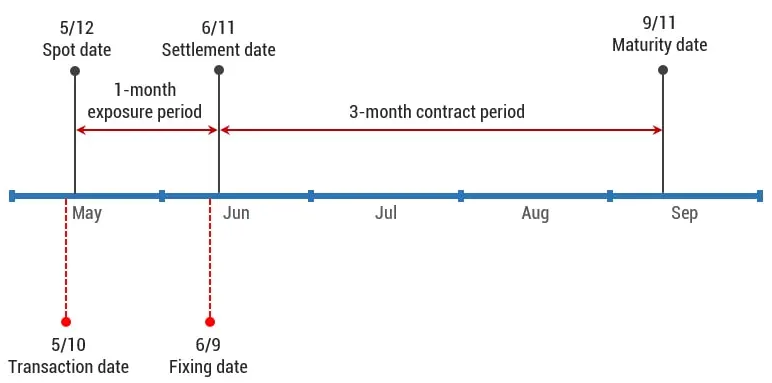
\includegraphics[width=0.8\linewidth]{fra_timeline}
	\end{center}
\end{itemize}
\end{frame}

\begin{frame}{FRA: Formalization of the Contract}
	\begin{itemize}
		\item<1-> Formally, at time $S$ one receives $\tau(T, S)KN$ units of currency and pays the amount $\tau(T,S)L(T,S)N$, where $N$ is the contract nominal value.
		\item<2-> Thus, at time $S$, the future (and \textbf{today unknown}) payout of the contract is: 
		\begin{equation}
			N\tau(T,S)(K-L(T,S))
			\label{eq:fra_payoff}
		\end{equation}
		\item<3-> In order to assign a value at this contract we have to tackle two issues:
		\begin{itemize}
			\item<4-> estimate the future value of $L(T, S)$;
			\item<5-> discount the result from $S$ to today (time $t$).
		\end{itemize}
		\item<6-> There are several ways to arrive at the final result: \textbf{no arbitrage is the common denominator.}
	\end{itemize}
\end{frame}

%\begin{frame}{FRA: Numerical Example}
%	A company enters into a FRA to receive 4\% on \$100M for a 3-month period starting in 3 years. Imagine that LIBOR is 4.5\% in 3 years.
%	
%	So $T=3y$, $S=3.25y$, $K=4\%$, and $L(T,S)=4.5\%$.
%	
%	The net cash-flow at time $S$ is
%	\begin{equation*}
	%		100000000\times(0.04-0.045)\times0.25 = -\$125000
	%	\end{equation*} 
%\end{frame}

\subsection{FRA Valuation}
\begin{frame}{FRA: Brigo-Mercurio Approach}
	\begin{itemize}
		\only<1-1>{
		\item Substitute in \cref{eq:fra_payoff} $L(T,S)$ with its expression as a function of the zero-coupon bond price $P$ and get
		\begin{equation*}
			N\bigg[\tau K + 1 - \frac{1}{P(T, S)}\bigg]
		\end{equation*}
		}
		\only<2->{
		\item Substitute in \cref{eq:fra_payoff} $L(T,S)$ with its expression as a function of the zero-coupon bond price $P$ and get
		\begin{equation*}
			N\bigg[\tau K + 1 - \underbrace{\frac{1}{P(T, S)}}_{A}\bigg]
		\end{equation*}
		}
		\item<2-> First interpret $A$ as an amount of money held at time $S$. At $T$ it's worth 1, indeed 
		\begin{equation*}
			A = P(S,S)A \implies P(T,S)A = P(T,S)\frac{1}{P(T,S)}=1
		\end{equation*}
		which in turn, at time $t$, equals to
		\begin{equation*}
			P(t,T) 1 = P(t,T)
		\end{equation*}
	\end{itemize}
\end{frame}

\begin{frame}{FRA: Brigo-Mercurio Approach}
	\begin{itemize}
		\item Substitute in \cref{eq:fra_payoff} $L(T,S)$ with its expression as a function of the zero-coupon bond price $P$ and get
		\begin{equation*}
			N\bigg[\underbrace{\tau K + 1}_{B} - \underbrace{\frac{1}{P(T, S)}}_{A}\bigg]
		\end{equation*}
		\item<1-> On the other hand $B$ in $S$ becomes at time $t$:
		$P(t,S)\tau K + P(t, S)$.
		\item<2-> Collecting the terms we get
		\begin{equation}
			\textbf{FRA}(t,T,S,\tau,N,K)=N[P(t,S)\tau K–P(t,T)+P(t,S)]
		\end{equation}
			\myendproof
	\end{itemize}
\end{frame}

\subsection{FRA Detailed Proof}
\begin{frame}{FRA Detailed Proof}
\begin{itemize}
	\item<1-> Let's start from the risk neutral pricing formula
	\begin{equation} \textbf{FRA} = 
\expectt{Q}{t}[\tau D(t,S)(K - L(T,S))] = 	\expectt{Q}{t}[\tau D(t,S)K - \tau D(t,S)L(T,S)]
	\label{eq:fra_as_expectation}
	\end{equation}
	To ease the notation $\expectt{Q}{t}[X] = \expectt{Q}{t}[X|\mathcal{F}_t]$.
	\item<2-> From which we can easily derive using the definition of \textbf{ZCB} value
	\begin{equation*}
		\begin{aligned}
		\textbf{FRA} = \tau &K\expectt{Q}{t}[D(t,S)] - \expectt{Q}{t}[\tau D(t,S)L(T,S)] = \\
		&=\tau KP(t,S) - \expectt{Q}{t}[\tau D(t,S)L(T,S)]
		\end{aligned}
	\end{equation*}
	\item<3-> For a discount factor the following holds
	\begin{equation*}
		D(t,S) = D(t,T)D(T,S)
	\end{equation*}
\end{itemize}
\end{frame}

\begin{frame}{FRA Detailed Proof}
	\begin{itemize}
		\item<1-> So we get
		\begin{equation*}
			\textbf{FRA} = \tau KP(t,S)-\expectt{Q}{t}[\tau D(t,T)D(T,S)L(T,S)]
		\end{equation*}
		\item<2-> Then using the tower expectation property
		\begin{equation*}
		\textbf{FRA} = \tau KP(t,S) - \expectt{Q}{t}[\mathbb{E}_T[\tau D(t,T)D(T,S)L(T,S)]]
		\end{equation*}
		\item<3-> Last equation can be transformed as
		\begin{equation*}
			\textbf{FRA} = \tau KP(t,S) - \expectt{Q}{t}[\tau D(t,T)L(T,S)\mathbb{E}_T[D(T,S)]]
		\end{equation*}
		\item<4-> From which
		\begin{equation*}
		\textbf{FRA} = \tau KP(t,S) - \expectt{Q}{t}[\tau D(t,T)L(T,S)P(T,S)]
		\end{equation*}
	\end{itemize}
\end{frame}

\begin{frame}{FRA Detailed Proof}
	\begin{itemize}
		\item<1-> Then using the definition of LIBOR rate $L(t,T)=\frac{(1-P(t,T))}{\tau(t,T)P(t,T)}$
		\begin{equation*}
			\begin{aligned}
			\textbf{FRA} = &\tau KP(t,S)-\expectt{Q}{t}\left[D(t,T)P(T,S)\left(\frac{1}{P(T,S)}-1\right)\right]= \\
			&=\tau KP(t,S)-\expectt{Q}{t}[D(t,T)] + \expectt{Q}{t}[D(t,T)P(T,S)]
			\end{aligned}
		\end{equation*}
		\item<2-> The last term can be expressed in terms of $D$
		\begin{equation*}
			\textbf{FRA} = \tau KP(t,S)-\expectt{Q}{t}[D(t,T)] + \expectt{Q}{t}\left[D(t,T)\expectt{Q}{T}[D(T,S)]\right]
		\end{equation*}		
		\item<2-> Bringing the discount factor inside the expectation
		\begin{equation*}
			\begin{aligned}
			\textbf{FRA} = &\tau KP(t,S)-\expectt{Q}{t}[D(t,T)] + 				\expectt{Q}{t}\left[\expectt{Q}{T}[D(t,T)D(T,S)]\right]=\\
			&=\tau KP(t,S)-\expectt{Q}{t}[D(t,T)] + \expectt{Q}{t}\left[\expectt{Q}{T}[D(t,S)]\right]
			\end{aligned}
		\end{equation*}		
	\end{itemize}
\end{frame}

\begin{frame}{FRA Detailed Proof}
	\begin{itemize}
		\item<1-> Then applying the law of iterated expectations we arrive at the final result
		\begin{equation*}
			\begin{aligned}
			\textbf{FRA} &= \tau KP(t,S)-\expectt{Q}{t}[D(t,T)] + 			\expectt{Q}{t}[D(t,S)] = \\
				&= \boxed{\tau KP(t,S) - P(t,T) + P(t,S)}
			\end{aligned}
		\end{equation*}
		\myendproof
	\end{itemize}
\begin{tikzpicture}[remember picture,overlay]
	\node[xshift=6.cm,yshift=-4.cm] (image) at (current page.center) {
\includegraphics[width=80px]{python}};
\end{tikzpicture}
\end{frame}

\subsection{Forward Rate Definition}
\begin{frame}{FRA: Forward Rate as Break-Even Rate}
	\begin{block}{Definition}
		The value of $K$ which makes the FRA worth zero is called \textcolor{red}{simply-compounded forward rate}
		\begin{equation}
			F(t;T,S):=\frac{1}{\tau(T,S)}\left[\frac{P(t,T)-P(t,S)}{P(t,S)}\right]
			\label{eq:forward_rate_definition}
		\end{equation}
	\end{block}
	
	The forward rate can be interpreted as a rate observed in $t$ and spanning the time period $S-T$.
	
	%Its value depends on no-arbitrage consideration.
	
\end{frame}

\begin{frame}{Forward Rate}
	\begin{itemize}
		\item We can now rewrite the value of the FRA in terms of the \emph{simply-compounded forward rate}
		\begin{equation}
			\begin{aligned}
			&\textbf{FRA}=N[\tau KP(t,S)-P(t,T)+P(t,S)] = \\
			&=N\tau P(t,S) \left[K +\frac{1}{\tau} \frac{P(t,S)-P(t,T)}{P(t,S)}\right] = N\tau P(t,S)(K-F(t;T,S))
			\end{aligned}
			\label{eq:fram_payoff_withF}
		\end{equation}
		(\textbf{note:} this formula will be used for the swap evaluation).
		\item<2-> Comparing to \cref{eq:fra_as_expectation} it is just like we had replaced the LIBOR rate $L(T,S)$ with the forward rate $F(t;T,S)$ in the payoff and then taken the present value of the (\emph{deterministic}) quantity.
		\item<3-> \textcolor{red}{The forward rate can be interpreted as an \emph{estimate} of the future spot rate}, which is unknown at time $t$ (random process based on the market conditions).
		\item<4-> \emph{We'll see later that indeed $F(t;T,S)$ is the expectation of $L(T,S)$ under a particular probability measure.}
	\end{itemize}
\end{frame}

\begin{frame}{Instantaneous Forward Rate}
	\begin{block}{Definition}
	The \textcolor{red}{instantaneous forward rate} $f(t, T)$ is defined as 
	\begin{equation}
		\begin{aligned}
			f(t, T) &:= \lim_{S\rightarrow T^+} F(t;T,S) \\
			& = \lim_{\epsilon\rightarrow 0}  \frac{1}{\tau(T,T+\epsilon)}\frac{P(t,T)-P(t,T+\epsilon)}{P(t,T+\epsilon)} \\
			& = \lim_{\epsilon\rightarrow 0} - \frac{1}{P(t,T)} \frac{P(t,T+\epsilon)-P(t,T)}{\epsilon} \\
			& = -\frac{\partial \log P(t, T)}{\partial T}
		\end{aligned}
	\end{equation}
	\end{block}
\end{frame}

\begin{frame}{Instantaneous Forward Rate}
	\begin{itemize}
		\item From the previous equation we can derive
		\begin{equation}
			P(t, T) = e^{-\int_t^T f(t, s) ds}
		\end{equation}
		\item The \emph{instantaneous forward rate} represents the rate for a forward contract with an infinitesimal investment period after the settlement date.
		\item Notice that
		\begin{equation*}
			r(t) = f(t,t)
		\end{equation*}
	\end{itemize}
\end{frame}

\begin{frame}{Homework}
\begin{itemize}
\item The 1-year spot rate on US treasury bonds is 9\%, the 2-year spot rate is 9.5\% and the 3-year spot rate is 10\%. 
\begin{itemize}
\item Calculate the implied 1-year ahead, 1-year forward rate, $F(0;1,2)$. Explain why a 1-year forward rate of 9.6\% could not be explained by the market;
\item calculate the forward rates  $F(0; 2, 3$ and $F(0; 1,3)$. Is there a link between $F(0;1,2),F(0;2,3)$ and $F(0;1,3)$ ?
\end{itemize}
\item A bank offers to borrow €100 from you at an interest rate applicable between the end of year 1 and the end of year 2 at a rate of 13\% (i.e. the forward rate). The spot rates for 1-year and 2-year are currently 10\% and 12\% respectively. Explain whether you would take the bank’s offer. 
\end{itemize}
\end{frame}

\section{Interest Rate Swap}
\begin{frame}{Interest Rate Swap}
	\begin{itemize}
		\item An \textcolor{red}{Interest Rate Swap} (IRS) is a contract that exchanges payments between two differently indexed \emph{legs}, starting from a future time. At every pre-specified instant $T_i$, the \emph{fixed leg} pays the amount ($N$ is the contract nominal)
		\begin{equation*}
			N\tau(T_{i-1}, T_i)K
		\end{equation*}
		while the \emph{variable leg} pays the amount
		\begin{equation*}
			N\tau(T_{i-1}, T_i)L(T_{i-1}, T_i)
		\end{equation*}
		\item<2-> When the fixed leg is paid, the IRS is termed \textcolor{red}{Payer IRS}. If the opposite holds, we have a \textcolor{red}{Receiver IRS}.
		\item<3-> The discounted payoff of a Payer IRS can be expressed as:
		\begin{equation}
			\sum_{i=\alpha+1}^{\beta} D(t,T_i)N \underbrace{\tau_i}_{\tau(T_{i-1},T_i)}
			\left[L(T_{i-1},T_i)-K\right]
			\label{eq:payoff_payer_irs}
		\end{equation}	
	\end{itemize}
\end{frame}

\begin{frame}{Interest Rate Swap}
\begin{center}
	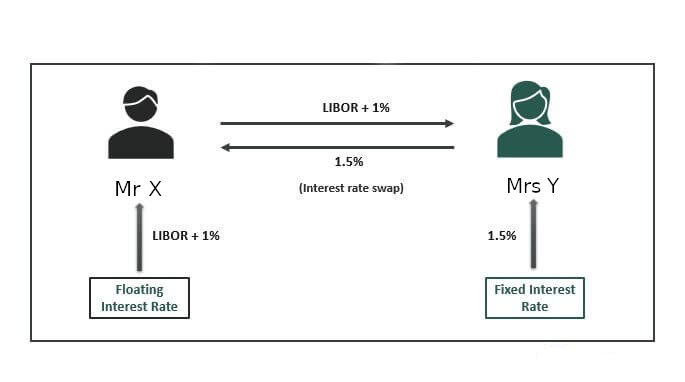
\includegraphics[width=0.9\linewidth]{Interest-Rate-Swap-diagram}
\end{center}
\end{frame}

\begin{frame}{IRS and FRA}
	\begin{itemize}
		\item The swap payoff in \cref{eq:payoff_payer_irs} can be re-interpreted as a portfolio of FRAs.
		\item Indeed consider a Receiver IRS and express its payoff as a sum of FRAs using \cref{eq:fram_payoff_withF}
		\begin{equation}
			\begin{aligned}
				\textbf{RFS}&(t,T,\tau,N,K) = 	N\sum_{i=\alpha+1}^{\beta}\expect{Q}[D(t,S)\tau_i(K - L(T_{i-1},T_i))]=\\
				&=N\sum_{i=\alpha+1}^{\beta}\tau_i P(t,T_i)(K-F(t;T_{i-1},T_i))\\
				&=N\sum_{i=\alpha+1}^{\beta}\tau_i KP(t,T_i)-N\sum_{i=\alpha+1}^{\beta}(P(t,T_{i-1})-P(t,T_i)) \\
				&=\boxed{N\sum_{i=\alpha+1}^{\beta}\tau_i KP(t,T_i)-NP(t,T_\alpha)+NP(t,T_\beta)}
			\end{aligned}
		\label{eq:swap_as_sum_fra}
		\end{equation}
	\end{itemize}
\end{frame}

\begin{frame}{IRS and FRA}
	\begin{itemize}
		\item<1-> Clearly not all the FRAs in a swap with zero value have zero value (\emph{except for the degenerate case of flat yield curve}): some of them will have positive NPV, some other negative; the only constraint being their sum to be zero.
		\item<2-> In a \emph{Payer Swap} with an increasing yield curve the first FRAs will have negative value, the last positive. Still their NPV's sum is zero.
		\item<3-> If the market doesn't move so much the swap rate payer will have to pay a net interest differential in the first part of the contract life, and to receive net interest in the second.
		\item<4-> So the rate payer will have to fund the payments for the first part of the contract and to invest at his best the receipt during the second part. (This is a very hot topic nowadays; this feature is sometimes referred to as the funding profile of the contract).
	\end{itemize}
	\uncover<4->{
		\begin{tikzpicture}[remember picture,overlay]
		\node[xshift=5cm,yshift=-3.7cm] (image) at (current page.center) {
\includegraphics[width=80px]{python}};
	\end{tikzpicture}}
\end{frame}

\begin{frame}{Homework}
\begin{itemize}
\item A 100 million interest rate swap has a remaining life of 10 months. Under the terms of the swap; 6-month LIBOR is exchanged for 7\% per annum (compounded semiannually). The average of the bid-offer rate being exchanged for 6-month LIBOR in swaps of all maturities is currently 5\% per annum with continuous compounding. The 6-month LIBOR rate was 4.6\% per annum 2 months ago. What is the current value of the swap to the party paying floating ? What is its value to the party paying fixed ?
\item Assume that company A has agreed to pay a 6-month Libor and receive a fixed interest rate of 8\% per annum (with interest payable every six months) from the face value of 100 million. Swap is 1.25 years to expire. The interest rates for 3, 9 and 15 months are: 10\%, 10.5\% and 11\% respectively. Assume that interest rates are continously compounded. The 6-month Libor is currently 10.2\%. Calculate the value of this swap for company A.
\item Determine the value of the swap from previous exercise in the way as described in the Relationship between interest rate swap and FRA part.
\end{itemize}
\end{frame}

\subsection{Swap Rate}
\begin{frame}{Swap Rate as Break-Even Rate}
	\begin{block}{Definition}
	The fixed rate $K$ which makes the above expression null is called \textcolor{red}{forward swap rate}:
	\begin{equation}
		S_{\alpha,\beta}(0) = \frac{P(0, T_\alpha)-P(0,T_\beta)}{\sum_{i=\alpha+1}^{\beta}\tau_iP(0,T_i)}
	\end{equation}
	If $T_\alpha=0$ we have the \textcolor{red}{spot swap rate} (which is published on financial newspapers).
	\end{block}
	The swap rate makes the contract fair at inception by definition.
\end{frame}

\begin{frame}{Swap Payoff Alternative Expression}
	\begin{itemize}
		\item<1-> Consider a Payer IRS with $N=1$ (using \cref{eq:swap_as_sum_fra})
		\begin{equation*}
			\textbf{PFS} = P(t,T_\alpha)-P(t,T_\beta)-\sum_{i=\alpha+1}^{\beta}\tau_iKP(t,T_i)
		\end{equation*}
		\item<2-> By multiplying and dividing by (the so called \textcolor{red}{annuity}) $A = \sum_{i=\alpha+1}^{\beta}\tau_iP(t, T_i)$
		we get
		\begin{equation}
			\begin{gathered}
			\textbf{PFS}=\frac{A}{\sum\tau_iP(t, T_i)}\left[P(t,T_\alpha)-P(t,T_\beta)-K\sum_{i=\alpha+1}^{\beta}\tau_i P(t,T_i)\right]=\\
			= \boxed{A (S_{\alpha,\beta}(t)-K)}
			\end{gathered}
		\label{eq:swap_payoff_with_swap_rate}
		\end{equation}
		(\textbf{note:} this expression will be useful when pricing swaptions).
	\end{itemize}
\end{frame}

\subsection{Swap and Bond Switching}
\begin{frame}{Swap and Bond Switching}
	\begin{itemize}
		\item<1-> Consider again a Payer Forward Swap (this time with notional $N$)
		\begin{equation*}
			\textbf{PFS}(t,T_\alpha,T_\beta,\tau,N,K)=N(P(t,T_\alpha)-P(t,T_\beta))-NK\sum_{i=\alpha+1}^{\beta} \tau_iP(t,T_i)
		\end{equation*}
		\item<2-> A swap can be considered as an exchange between two kinds of bond with the same notional reimbursed at maturity. In fact:
		\begin{itemize}
		 \item<3->\emph{the fixed leg} of the swap can be viewed as a \textcolor{red}{fixed coupon stream};
		 \item<4-> while the \emph{variable} can be considered a \textcolor{red}{floating rate note coupon stream}. 
		\end{itemize}
%		\item When $T_\alpha = t$, i.e. we take the particular case of spot trading (PFS becomes...PS). We thus get
%		\begin{equation*}
%			\begin{aligned}
%				\text{PS}(t,T_\beta) &=N-\underbrace{NP(t,T_\beta)}_{\text{notional exch.}}-\underbrace{KN\sum_{i=\alpha+1}^{\beta} \tau_iP(t,T_i)}_{\text{coupons exch.}} \\
%				&=N-\textbf{CBP}(t,T_\beta,K,N)
%			\end{aligned}
%		\end{equation*}
	\end{itemize}
\end{frame}

\begin{frame}{Fixed Rate Side}
	\begin{itemize}
		\item<1-> Consider a coupon bond that pays the following cash flows $\mathcal{C}=\{c_{\alpha+1},\ldots,c_\beta\}$ on the schedule $\mathcal{T} = \{T_{\alpha+1},\ldots,T_\beta\}$ with 
		\begin{equation*}
			\begin{cases}
				c_i = N\tau K,\quad i<\beta \\
				c_\beta=N\tau K+N, \quad i=\beta	
			\end{cases}		
		\end{equation*}
		\item<2-> The coupon bond price can be written as the discounted sum of the cash-flows
		\begin{equation}
			\textbf{CBP}(t,\mathcal{C},T)=\sum_{i=\alpha+1}^{\beta}c_i P(t,T_i)
		\end{equation}
		\item<3-> Needless to say that in case $K=0$ the bond reduces to a zero-coupon bond with maturity $T_\beta$.
		
%		\item Last equation rearranged gives
%		\begin{equation}
%			\textbf{CBP}(t,T_\beta,K,N) = N - PS(t,T_\beta)
%		\end{equation}
	\end{itemize}
%	\begin{block}{Intepretation}
%		The meaning is pretty straightforward: a fixed rate bond can be replicated using the NPV of a payer swap whose fixed leg coincides with the fixed leg of the bond. The floating leg represents the funding of the bond, i.e. the interests the issuer must pay to raise funds in the interbank market when his spread over the benchmark LIBOR rate is null.
%	\end{block}
\end{frame}

%\begin{frame}{Swap and Bond Switching}
%	\begin{itemize}
%		\item More formally, consider a coupon bond that pays the following cash flows $\mathcal{C}=[c_{\alpha+1},\ldots,c_\beta]$	on the schedule $T = [T_{\alpha+1},\ldots,T_\beta]$ with 
%		\begin{equation*}
%			\begin{cases}
%			c_i = N\tau K,\quad i<\beta \\
%			c_\beta=N\tau K+N, \quad i=\beta	
%			\end{cases}		
%		\end{equation*}
%		\item The coupon bond price can be written as
%		\begin{equation}
%			\textbf{CBP}(t,\mathcal{C},T)=\sum_{i=\alpha+1}^{\beta}c_i P(t,T_i)
%		\end{equation}
%	\end{itemize}
%\end{frame}

\begin{frame}{Floating Rate Note (FRN)}
	\begin{itemize}
		\item<0-> Next consider a floating rate note that pays coupons at dates
		\begin{equation*}
			\mathcal{T}_{\text{payments}} = \{T_{\alpha+1},\ldots,T_\beta\}
		\end{equation*}
		coupons calculated at the LIBOR rate fixed in the previous period
		\begin{equation*}
			\mathcal{T}_{\text{fixings}} = \{T_{\alpha},\ldots,T_{\beta - 1}\}
		\end{equation*}
		\item<1-> At maturity $T_\beta$ the notional is reimbursed as before.
		\item<2-> To value this note we change sign to the \textbf{RFS} (\cref{eq:swap_as_sum_fra}), set $K=0$, i.e. no fixed rate payments are done, and finally add the present value of the notional at maturity: $NP(t,T_\beta)$
		\begin{equation*}
			\begin{aligned}
			\textbf{FRN} &= -\textbf{RFS} + NP(t,T_\beta) =\\
			& =NP(t,T_\alpha)-NP(t,T_\beta)-N\sum_{i=\alpha+1}^{\beta}K\tau_i P(t,T_i) + NP(t,T_\beta)
		\end{aligned}
		\end{equation*}
	\end{itemize}
\end{frame}

\begin{frame}{Floating Rate Note (FRN)}
	\begin{itemize}
		\item Next consider a floating rate note that pays coupons at dates
		\begin{equation*}
			\mathcal{T}_{\text{payments}} = \{T_{\alpha+1},\ldots,T_\beta\}
		\end{equation*}
		coupons calculated at the LIBOR rate fixed in the previous period
		\begin{equation*}
			\mathcal{T}_{\text{fixings}} = \{T_{\alpha},\ldots,T_{\beta - 1}\}
		\end{equation*}
		\item At maturity $T_\beta$ the notional is reimbursed as before.
		\item To value this note we change sign to the \textbf{RFS} (\cref{eq:swap_as_sum_fra}), set $K=0$, i.e. no fixed rate payments are done, and finally add the present value of the notional at maturity: $NP(t,T_\beta)$
		\begin{equation*}
		\begin{aligned}
			\textbf{FRN} &= -\textbf{RFS} + NP(t,T_\beta) =\\
			& =NP(t,T_\alpha)-\cancel{NP(t,T_\beta)}-\cancel{N\sum_{i=\alpha+1}^{\beta}K\tau_i P(t,T_i)} + \cancel{NP(t,T_\beta)} =NP(t,T_\alpha)
		\end{aligned}
		\end{equation*}
	\end{itemize}
\end{frame}

\begin{frame}{Floating Rate Note (FRN)}
	\begin{itemize}
	\item The intuition behind this formula is quite straightforward: if we set $T_\alpha =t$. \textcolor{red}{At the date of the first reset, the bond price equals par.} 
	\item This result also holds for all the dates equal to the reset of the floating rates (an \textbf{FRN} is equivalent to a roll-over strategy of short-term loans).
	\item This property is sometimes summarized by the sentence "the \textbf{FRN} always trade at par".
	\item The \textbf{FRN} is a debt security in which coupon payments adjust according to changes in interest rates. The coupons are closely tied to current short-term spot rates, such that their prices are always at or near par value (no arbitrage). 
	%\item Provide an example of Italian government floating rate note. Did they trade at par in recent times ? Provide an explanation.
	\end{itemize}
	\begin{tikzpicture}[remember picture,overlay]
	\node[xshift=5cm,yshift=-3.7cm] (image) at (current page.center) {
\includegraphics[width=80px]{python}};
\end{tikzpicture}
\end{frame}

\subsection{Fixed vs Variables}
\begin{frame}{Concepts behind the Formulas}
	Suppose that a generic bank, \emph{MyFavouriteBank}, has the same credit risk of the corresponding average inter-bank entity. So, \textcolor{red}{the spread over the LIBOR rate is 0}. Suppose now the bank needs financing and it plans to issue coupon bonds. It has two alternatives:
	\begin{enumerate}
		\item<1-> borrow $N$ and pay floating interests at the rates
		\begin{equation*}
			L(T_{i-1},T_i);
		\end{equation*}
		\item<2-> borrow $N$ and pay fixed interests given by the coupon
		\begin{equation*}
			K = S_{\alpha,\beta}.
		\end{equation*}
		(clearly the overall cost to raise money must be the same at the beginning, i.e. fixed leg NPV equals floating leg NPV).
	\end{enumerate}
\end{frame}

\begin{frame}{Concepts behind the Formulas}
	\begin{itemize}
		\item<1-> Given the two strategies are equivalent the bank will then opt for one of two alternatives depending on:
		\begin{enumerate}
			\item marketing considerations, i.e. which kind of bond people prefer;
			\item the interest rate risk it wants to have.
		\end{enumerate} 
		\item<2-> Remember that a variable rate mortgage is perceived risky by the average individual as salary is more or less fixed, but for bank this is not the case because it is left unarmed by the rate rise. Indeed if rates go up
		\begin{itemize}
			\item the bank loses in the higher coupons it has to pay to the bond holders;
			\item the bank gains in the highest rates it charges on new loans at the same time.
		\end{itemize}
		\item<3-> This is the most basic example of \emph{asset liability matching}.
		\item<4-> The same more or less holds for a rate decrease.%, but with some caveats.
	\end{itemize}
\end{frame}

\begin{frame}{Concepts behind the Formulas}
	\begin{itemize}
		\item<0->Banks like floating rates exposure: 
		\begin{itemize}
			\item<1-> [\goodcheck] the liability value (the bond floating rate) resets with rates;
			\item<1-> [\goodcheck] often smaller costs then fixed rates;
			\item<1-> [\goodcheck]surely less expensive in the case of a long-term loan (e.g. 30-year mortgage), lenders require higher fixed rates in that case, due to bad accuracy in forecast economic conditions over such a long period of time.
		%\end{itemize}
		%\begin{itemize}
			\item<2-> [\badcheck] higher interest rate risk (risk of rising rates in the future);
			\item<2-> [\badcheck] with inverted yield curve, the cost of debt may actually be higher than fixed-rate debt (however, this is the exception rather than the norm).
		\end{itemize}
% There is a general assumption that interest rates will rise – or, increase – over time,
	\end{itemize}
\end{frame}

\begin{frame}{Concepts behind the Formulas}
	\begin{itemize}
		\item<1-> So why do not banks issue only floating rate notes ?
		\item<2-> Banks must issue fixed rate coupon bonds to attract customers (think of yourself or insurance companies) but then will hedge the liability  with an investment bank. In this way the final risk exposure will be at a variable rate as they like. 
		\item<3-> \textcolor{red}{Swaps are both a hedging instrument and a pricing tool.}
	\end{itemize}
\end{frame}

\subsection{Basis Swaps}
\begin{frame}{Basis Swap}
	\begin{itemize}
	\item A \textcolor{red}{(Tenor) Basis Swap} is defined as a contract in which two floating legs are exchanged.
	\item The two legs can differ both in the tenor of the underlying rate and in the frequency of payments.
	\item For instance a typical Basis Swap is one in which a floating leg indexed to EURIBOR-6M is exchanged against one indexed to EURIBOR-3M.
	\end{itemize}
	\begin{center}
		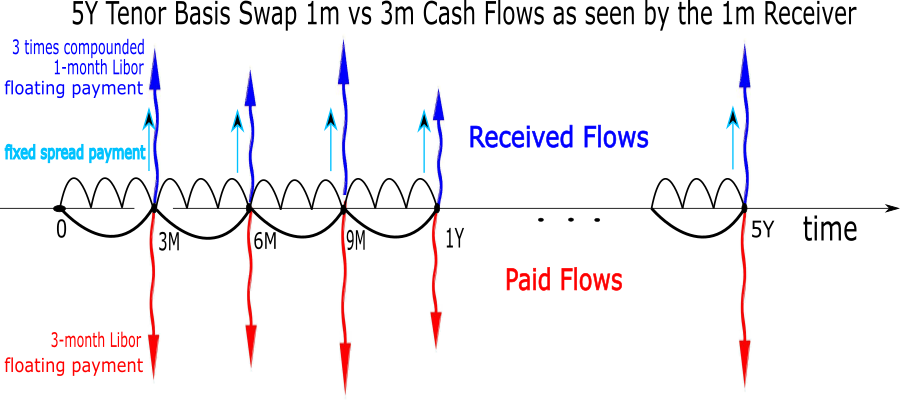
\includegraphics[width=0.5\linewidth]{tenor_basis_swap}
	\end{center}
\end{frame}

\begin{frame}{Basis Swap Valuation}
\begin{itemize}
	\item<1-> A Tenor Basis Swap can be priced according to the following
	\begin{equation}
	\textbf{TBS}(t) = \sum_{i=1}^n \tau_i^{L} F^{L}(t;T_{i-1},T_i)P(t,T_i) - \sum_{j=1}^m \tau_j^{S} (F^{S}(t;T_{j-1},T_j)+s)P(t,T_j)
	\end{equation}
	where $L$ (long index) denotes the index with the longer tenor and $S$ (short index) the other with the shorter tenor.
	\item<2-> Basis Swaps usually quote at par, meaning that the price of the swap is zero and that the present value (PV) of each of the traded legs is the same. 
	\item<3-> This is made possible by adding a \textcolor{red}{basis spread $s$} to the Ibor index with the lower frequency tenor.
	\end{itemize}
\end{frame}

\begin{frame}{Basis Swap Spread}
	\begin{itemize}
	\item But according to the \textcolor{red}{single curve framework} there should be no basis as the value of the floating leg
	is given by (forward start case)s
	\begin{equation*}
	P(0, T_0) - P(0, T_n)
	\end{equation*}
	or the following (spot case)
	\begin{equation*}
	1 - P(0, T_n)
	\end{equation*}
	(assuming $N=1$).
	\begin{columns}
	\column{0.4\linewidth}
	\item In both cases what matters are the first reset date and the last payment date; hence if they are the same for the two legs (regardless the reset frequency and the index tenor), the basis should be zero.
	\column{0.5\linewidth}
		\begin{center}
		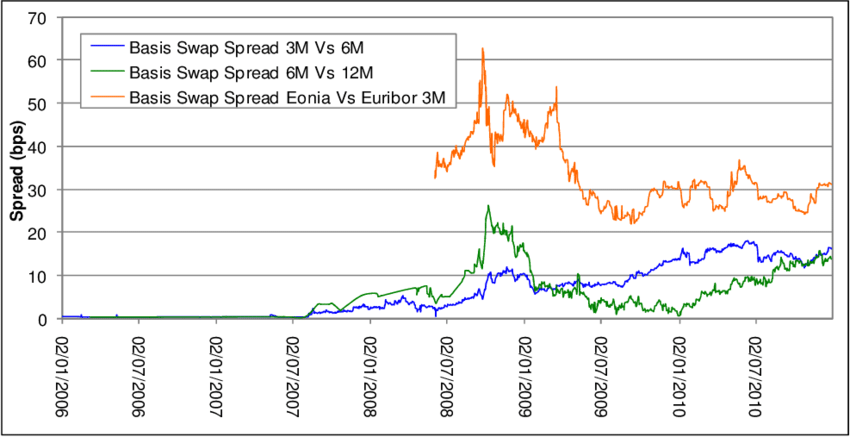
\includegraphics[width=1.\linewidth]{Basis-Swap-spreads-Euribor-3M-Vs-Euribor-6M-Euribor-6M-Vs-Euribor-12M-and-Eonia-Vs}
		\end{center}
	\end{columns}
	\end{itemize}
	%Exercise: write in detail the above argument, and provide an example for both a 10Y spot start basis swap and a 1Y forward 10Y Swap. Which condition you need to derive the result?
\end{frame}

\section{Credit Risk and Asset Swap}
\begin{frame}{Adding Credit Risk}
	\begin{itemize}
		\item When we make the real world enter the picture, a typical bank will pay a spread over LIBOR representing the \textcolor{red}{credit risk} (and other stuff, but leave this extra aside for the moment). 
		%\item For the swap to be worth 0 at inception the fixed rate must be higher as well. 
		\item<2-> Hence a bank which has credit risk will have to pay
		\begin{enumerate}
			\item a higher coupon if it issues a bond with fixed coupon;
			\item a spread over the variable rate if it opts for a floating rate bond.
		\end{enumerate}
		\item<3-> Often, in the first case, it will swap the liability, i.e. the bank is liable towards the bond holders, to hedge the pure rate risk. 
		\item<4-> This lead us to the next topic, the Asset Swap (and the asset swap spread).
	\end{itemize}
\end{frame}

\begin{frame}{Par Asset Swap}
	\begin{itemize}
		\item<1-> An \textcolor{red}{Asset Swap} (AS) can be defined as a \emph{synthetic floating-rate note}.
		\item In fact, the Asset Swap transforms a fixed rate into a floating one, \textcolor{red}{leaving the credit risk profile unchanged}.
		\item<1-> In the following we are going to consider \textcolor{red}{Par Asset Swaps}. 
		\item<2-> The package is made of a position in a bond and another in a swap.
		\item<3-> In case of \textcolor{red}{default} of the bond issuer, the Asset Swap buyer \textcolor{red}{must pay the fixed leg and the principal in the swap} but \textcolor{red}{does not receive the coupon} of the defaulted bond. 
	\end{itemize}
\end{frame}

\begin{frame}{Valuation of the Asset Swap}
	\begin{center}
		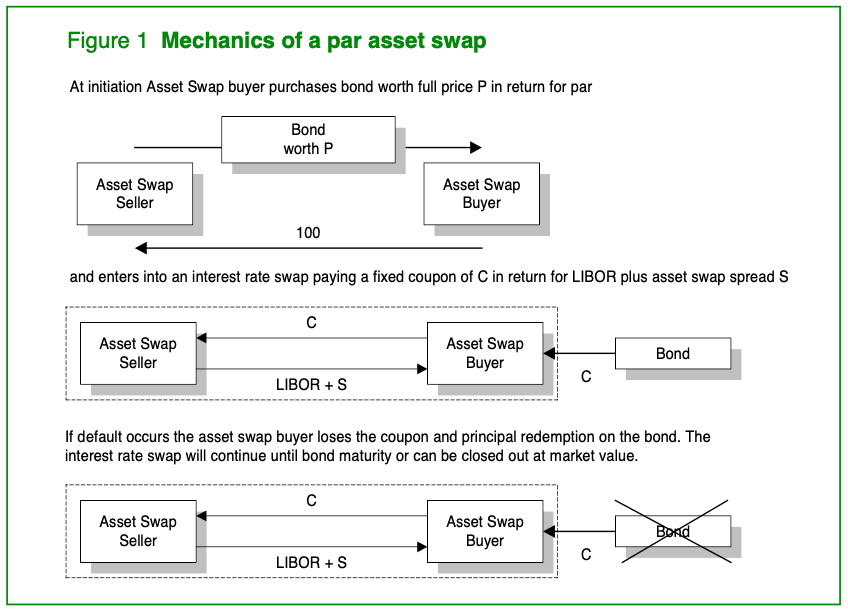
\includegraphics[width=0.7\linewidth]{asset_swap}
	\end{center}
\end{frame}

\subsection{Asset Swap Valuation}
\begin{frame}{Valuation of the Asset Swap}
	At valuation time $t$ the \emph{three} following facts are observed:
	\begin{itemize}
		\item<2-> the AS buyer buys a generic \emph{risky} coupon bond at the market price $\overline{\textbf{CBP}}(t,T,K,1)$;
		\item<3-> the AS seller pays/receives to/from the asset swap buyer the difference $\Delta = \overline{\textbf{CBP}}(t,T,K,N)-1$ in such a way that the net sum paid from the AS buyer is always 1; 
		\begin{itemize}
			\item \textcolor{red}{if the bond trades above par} the difference $\Delta$ is paid to the AS buyer by the seller;
			\item conversely \textcolor{red}{if the bond trades below par} the difference $\Delta$ is paid to the AS seller by the buyer.
		\end{itemize}
		\item<4-> A swap is then started between the two counter-parties such that the AS seller receives a fixed leg equal to the coupon stream of the bond and the AS buyer receives the floating leg given by LIBOR rate plus a \textcolor{red}{spread ($s$)}.
	\end{itemize}
\end{frame}

\begin{frame}{Valuation of the Asset Swap}
	\begin{itemize}
		\item From the perspective of the Asset Swap seller the value of the package is given by (we are considering spot trading so $T_\alpha = t = 0$)
		\begin{equation}
			\begin{aligned}
				\textbf{AS}=1&-\overline{\textbf{CBP}}+K\sum_{i=1}^{\beta}\tau_i P(0,T_i)-\sum_{i=1}^{\beta}\tau_i P(0,T_i)(L(T_{i-1},T_i)+s) =\\
				=1&-\overline{\textbf{CBP}}+K\sum_{i=1}^{\beta}\tau_i P(0,T_i)\\
				&-\sum_{i=1}^{\beta}\tau_i P(0,T_i)L(T_{i-1},T_i)-\sum_{i=1}^{\beta}\tau_i P(0,T_i)s=0
			\end{aligned}
			\label{eq:asset_swap_value}
		\end{equation}
	\end{itemize}
\end{frame}

\begin{frame}{Valuation of the Asset Swap}
	\begin{itemize}
		\item We can replace the future rates with the forward rates, and by its definition (\cref{eq:forward_rate_definition})
		\begin{equation*}
			\begin{aligned}
			&\sum_{i=1}^\beta \tau_i P(0,T_i)F(t;T_{i-1},T_i) =  \sum_{i=1}^\beta \cancel{P(0,T_i)}\frac{P(0,T_{i-1})-P(0,T_i)}{\cancel{P(0,T_i)}} = \\
			&= P(0,0) \cancel{- P(0,T_1)} + \cancel{P(0,T_1)} \cancel{- P(0,T_2)} + \cancel{P(0,T_2)} + \\
			&\ldots \cancel{- P(0, T_{\beta-1})} \cancel{+ P(0, T_{\beta-1})}-P(0,T_\beta) = 1-P(0,T_\beta) 
			\end{aligned}
		\end{equation*}
		\item Substitute into \cref{eq:asset_swap_value} to get
		\begin{equation*}
			\begin{aligned}
				\textbf{AS}=1&-\overline{\textbf{CBP}}+K\sum_{i=1}^{\beta}\tau_i P(0,T_i) -(1-P(0,T_\beta))
				+ \sum_{i=1}^\beta\tau_i P(0,T_i)s=0
			\end{aligned}
		\end{equation*}
	\end{itemize}
\end{frame}

\begin{frame}{Valuation of the Asset Swap}
	\begin{itemize}
		\item Canceling out the 1s
		\begin{equation*}
			\begin{aligned}
				\textbf{AS}=&-\overline{\textbf{CBP}}+K\sum_{i=1}^\beta\tau_i P(0,T_i) +P(0,T_\beta) \\
				& + \sum_{i=1}^{\beta}\tau_i P(0,T_i)s=0
			\end{aligned}
		\end{equation*}
		\item Finally we know that
		\begin{equation*}
			K\sum_{i=1}^\beta\tau_i P(0,T_i) + P(0,T_\beta)
		\end{equation*}
		represents the price of coupons and principal of a  risk-free bond which can be denoted by \textbf{CBP}.
	\end{itemize}
\end{frame}

\subsection{Asset Swap Spread}
\begin{frame}{Asset Swap Spread}
	Solving for $s$ we arrive at the final expression
	\begin{equation}
		s = \frac{\textbf{CBP}-\overline{\textbf{CBP}}}{\sum_{i=1}^{\beta}\tau_iP(0,T_i)}
	\end{equation}
	\begin{itemize}
	\item<2-> An asset swap enables an investor to buy a fixed rate bond and then hedge out the interest rate risk by swapping the fixed payments to floating. In doing so the investor retains the credit risk of the bond but earns a corresponding return. 
	\item<3-> She is still exposed to the loss of the coupons and redemption on the bond, i.e. the difference between bond and recovery value.
	\item<4-> In economic terms the purpose of the Asset Swap Spread is to compensate the Asset Swap buyer for taking these risks, which is measured by the spread.
	\item<5-> If the credit worthiness of the issuer reduces ($\overline{\textbf{CBP}}$ decreases), rates remain constant, so $s$ increases.
	\end{itemize}
\end{frame}

\begin{frame}{Asset Swap: Credit Considerations}
	\begin {itemize}
%	\item If the bond defaults, the AS buyer has to continue paying on the swap, which can no longer be funded with the coupon from the bond, or the swap can be closed out at market value. The asset swap buyer also loses the par redemption of the bond, receiving whatever recovery rate the bond issuer pays. 
	\item A trader may want to hedge the credit risk carried on with the asset swap entering into a Credit Default Swap (CDS).
	\item A CDS is a credit insurance contract where the protection buyer pays \emph{spread} ($s_{CDS}$)and in case of a credit event, the protection seller must pay the contingency payment so that the buyer receives no losses from the default.
	\item Like $s_{AS}$, also $s_{CDS}$ is quoted on the market, tracking the perceived credit worthiness of the underlying reference entity.
	\item To avoid arbitrage opportunities, $s_{AS}$ of bond with maturity $T$ must be very close to corresponding maturity CDS spread $s_{CDS}$
	\begin{itemize}
		\item if $s_{AS} - s_{CDS} > 0$ the investor can buy the bond, financing the purchase, enters in AS and buying protection, making an (almost) risk free profit (\emph{negative basis trading});
		\item if $s_{AS} - s_{CDS} < 0$ can do the opposite.
	\end{itemize}
	\end{itemize}
	\begin{tikzpicture}[remember picture,overlay]
		\node[xshift=5cm,yshift=-3.7cm] (image) at (current page.center) {
\includegraphics[width=80px]{python}};
\end{tikzpicture}
\end{frame}

\begin{frame}{Homework}
\begin{itemize}
\item Describe the asset swap contract for a coupon bond with coupons equal to \textbf{C} and dirty Price equal to $P(t)$. What will happen to the price if the spread increase, all the rest being equal? What does it mean in term of credit quality expectation by the market for the bond's issuer?
\item  Consider the 10-year German Bund DBR 0.5\% 2026 which is currently trading at a clean price of 104.58. 
Given that the 10-year EUR swap rate is 0.44\% what is the par-par asset swap spread for this bond? 
For this exercise assume the all Annuity Factors have a value of 10.0 for simplicity.
\item Consider the 10-year Greek Government Bond GGB 3.0\% 2026 which is currently trading at a clean price of 75.280. Given that the 10-year EUR swap rate is 0.440\% what is the par-par asset swap spread for this bond?
\end{itemize}
\end{frame}

\section{Risk Measures}
\begin{frame}{Estimating Risk}
\begin{itemize}
\item After pricing a trader/investor computes Swap risk for hedging.
\item There are several metrics to assess the risk and different ways to measure their actual value:
\begin{itemize}
	\item \textbf{analytical}: involves deriving a closed-form solution which can be complex and is not always possible;
	\item \textbf{numerical}: one bumps the yield curve calibration instruments and reprice the swap. The change in price gives the risk;
	\item \textbf{curve Jacobians}: when yield curves have been calibrated, the solver slope 'Jacobian' can be kept and used to give the change in swap price for a change in forwards/discount factors;
	\item \textbf{algorithmic differentiation}: can be used to compute risk "automatically" at the same time as computing the price. It produces accurate and fast risk.
\end{itemize}
\end{itemize}
\end{frame}

%\begin{frame}{Delta Risk}
%	\begin{itemize}
%	\item<1-> The concept of delta risk on interest rate derivatives is a generalization of the traditional one of a single asset option. 
%	\item<2-> The delta risk measures precisely the risk associated with the shift of the interest rate curve. 
%	\item<3-> However there are a number of complications...
%	\item<4-> Interest rate derivatives depend on a variety of instruments, used in the determination of the interest rate curve, rather than a single asset.
%	\item<5-> Because there are many ways of shifting the interest rate curve, many different deltas can be computed. 
%	\end{itemize}
%\end{frame}

\begin{frame}{Basis Point Value}
\begin{itemize}
%	\item Consider the NVP of an IRS
%	\begin{equation*}
%	\textbf{NPV}=\sum_{i=\alpha+1}^\beta\tau_iP(t,T_i)(K-L(T_{i-1},T_i))
%	\end{equation*}
	\item<1-> The \textcolor{red}{Basis Point Value (BPV)} is computed by changing the value of the fixed coupon by 1~bp and evaluating the impact on the NPV. It is equal to the discounted value of the cash-flows for a rate of 0.01\% for all periods of the fixed leg
	\begin{equation}
	\textbf{BPV} = 0.01\% \frac{\partial \textbf{PFS}}{\partial K} = 0.01\% \sum_{i=\alpha+1}^\beta\tau_iP(t,T_i)
	\end{equation}
	\item<2-> This is a useful measure for dealers calculating the exact P\&L generated by applying a spread (or margin) to a fixed rate away from the mid-market rate.
\end{itemize}
\end{frame}

%%Ingoring for simplicity the fact that we now have different curves for discounting and projecting forward floating rates, LIBOR basis and what not, the PV of the floating leg of the swap is
%%PVfloat=1−𝑃(0,𝑇𝑛)(1)
%%(assuming again for simplicity that the swap starts today and 𝑃(0,𝑇𝑛)
%%is the discount factor from the swap maturity 𝑇𝑛
%%). Likewise, the PV of the fixed leg is
%%PVfix=∑𝑖=1𝑛𝐶𝑃(0,𝑇𝑖)(2)
%%where 𝐶
%%is the fixed rate in the swap. Assuming for simplicity annual payments.
%%
%%Theoretically, the interest rate risk of the swap is obtained by shifting each rate that was used to construct the discount factors 𝑃(0,𝑇𝑖)
%%then revaluing the swap and then taking the PV difference.
%
%%What Bloomberg seems to do instead is to calculate the new fixed PV by shifting the fixed rate 𝐶
%%. Even though it stays constant (it is a term of the trade) this is approximately valid because when all rates change that were used to construct the discount factors then in particular the fair swap rate for maturity 𝑇𝑛
%%will change. This fair swap rate is related to the discount factors by
%%𝐶fair=1−𝑃(0,𝑇𝑛)∑𝑛𝑖=1𝑃(0,𝑇𝑖)
%%which follows simply from PVfloat=PVfix

\begin{frame}{Basis Point Value}
\begin{itemize}
	\item<1-> Nevertheless BPV can also be used as an approximation for the interest rate risk.
	\item<1-> Indeed in the single-curve framework the "fair" Swap rate can be expressed as 
	\begin{equation*}
		K_{\text{fair}}=\frac{1-P(0, T_\beta)}{\sum_i P(0, T_i)}
	\end{equation*} 
	assuming for simplicity annual payments ($\tau = 1$) and that the Swap starts today.
	\item<2-> When perturbing the term structure, it turns out that $K_{\text{fair}}$ changes a lot more than the individual discount factors do. 
	\item<3-> Therefore, $NPV_{\text{float}}$ variation can be neglected and the total NPV variation can be approximated by
	\begin{equation*}
	\Delta\textbf{PS} = K'_{\text{fair}}\sum_i P(0, T_i) - K_{\text{fair}}\sum_i P(0, T_i) = \sum_i \underbrace{(K'_{\text{fair}} - K_{\text{fair}})}_{\text{typically few bps}}P(0, T_i) \end{equation*}
\end{itemize}
\end{frame}

\begin{frame}{PV01}
\begin{itemize}
\item PV01 measures the sensitivity of a Swap to a one basis point parallel shift in interest rates. Specifically it is defined as a Swap's fixed leg annuity scaled by 1~bp
\begin{equation}
PV01 = A/10000
\end{equation}
\item Numerically we can serve the PV01 by bumping the yield curve calibration instruments by 1~bp. 
%PV01 can be considered as the DV01 for par swaps (just set the fixed rate in the DV01 formula to the par rate making the PVswap term equal zero.
%par rate = swap equivalent of bond yield to maturity
\end{itemize}
\end{frame}

\begin{frame}{DV01}
\begin{itemize}
	\item<1-> If you want to know the \emph{linear} risk associated to a Interest Rate Swap if the market actually moves, you can make a slightly different calculation than above.
	\item<2-> The \textcolor{red}{Dollar value of a basis point (DV01)} refers to the exposure of a Swap position to a \textbf{down-shift} move of 1~bp in the forward rate curve.
	\item<3-> In the \emph{real} scenario the fixed rate is, well, fixed and floating rates move, so you can consider what happens to the NPV if every forecast rate $r_i$ are changed in parallel by the same amount
	\begin{equation*}
	\textbf{DV01} = \sum_j \frac{\partial \textbf{PFS}}{\partial r_j} = -\sum_{j}\tau_jP_j+\sum_{j}\left(K\sum_{i=\alpha+1}^\beta\tau_i\frac{\partial P_i}{\partial r_j} - \sum_{k=\alpha+1}^\beta L_k\tau_k\frac{\partial P_k}{\partial r_j}\right)
	\end{equation*}
	\item<4-> In the multi-curve framework DV01 would be calculated for the forecast curve, and for the discounting curve, resulting in two actual DV01 measurements.
\end{itemize}
%\begin{frame}{What does DV01 tell us ?}
%\begin{itemize}
%\item The DV01 calculates the profit or loss our swap will make from a down-shift in interest rates. 
%\item Specifically it calculates the P&L from a 1 basis point down-shift in both OIS rates, used to calculate discount factors, and Libor forecast rates. 
%\item The DV01 calculation is made up of a PV01 term, which indicates the risk to Libor forecast rates, and a DV01 add-on which indicates the risk to OIS discounting rates.
%\end{itemize}
%\end{frame}
\end{frame}

%Generally speaking an approximation for $\frac{\partial D_i}{\partial L_j}=\tau_i D_i$ if the rate $L_j$ impacts $D_i$ (i.e. if the rate is before $D_i$) and zero otherwise, so this is approximately:
%\begin{equation*}
%\frac{\partial \textbf{NPV}}{\partial r} = \underbrace{-\sum_{j}\tau_jD_j}_{\text{float leg}}+\underbrace{\sum_{j}\left(K\sum_{i=j}\tau_j\tau_iD_i - \sum_{k=j} L_k\tau_k\tau_j D_k\right)}_{\text{curvature and cashflows}}
%\end{equation*}

%If the schedules on the fixed and floating legs are the same, $i=j$, then you can see further similarity between the formulae. Additionally if the curve is flat, i.e. $L_j=K\forall j$ then the curvature component is zero.

\begin{frame}{DV01 Numerical Calculation}
\begin{itemize}
	\item<1-> Assume the P\&L on a Swap could be approximated by its linear P\&L plus its convexity
	\begin{equation*}
	\Delta \textbf{PFS}(\delta r)\approx \frac{\partial \textbf{PFS} }{\partial r}\delta r + \frac{1}{2}\frac{\partial^2 \textbf{PFS}}{\partial r^2}\delta r^2
	\end{equation*}
	\item<2-> Then bumping $\delta r$ by $\pm 1$~bp and dividing by 2 eliminates the convexity element and very accurately approximates the real DV01
	\begin{equation*}
	\textbf{DV01} = \frac{\Delta \textbf{PFS}(+1~bp)-\Delta \textbf{PFS}(-1~bp)}{2}=\frac{\partial \textbf{PFS} }{\partial r}
	\end{equation*}
	\item<3-> Another common method of calculation is to use a single bumped curve by, say, $\frac{1}{100}$th of a bp, and scale the result by 100 (less accurate, since the convexity is marginalised and not eliminated)
	\begin{equation*}
	100\Delta \textbf{PFS}\left(\frac{1}{100}~bp\right)=\frac{\partial \textbf{PFS}}{\partial r}+\frac{1}{200}\frac{\partial^2\textbf{PFS}}{\partial r^2}
	\end{equation*}
	\end{itemize}
\end{frame}

%\begin{frame}{DV01}
%\begin {itemize}
%\item It is common to calculate swap DV01 by decomposing the swap into a fixed and floating rate bond: DV01 becomes the sensitivity of a bond to a down-shift of 1 basis point in yield to maturity.
%\item Swap DV01 measures the sensitivity of a swap to changes in both forecast and discount curves. The Libor risk is usually much larger than the discount. % (except for swaps trading far from par). 
%\item Most of the risk comes from the floating leg since it is the only one sensitive to the forecast rate changes, while both carry discount risk.
%%Numerically it can be calculated by shifiting calibration instruments of both libor and ois discounting by 1 bp downwards. Heuristically this makes sence since the par rate by definition is the weighted average of libor forecast rates with OIS discount factors as weights.
%%Analytically DV01 can be calculated using \emph{modified duration approach}. Duration indicates the percentage chage in price for a percentage change in yield. DV01^{bond} = -B*D/10000 (B bond clean price).
%%Using bond interpretation a fixed rate receiver swap is a long bond and short a bond floater and vice versa for a receiver swap. 
%%The floating rate bond has no risk to forward rate changes, since floating coupons track Libor and are naturally immunized against interest rate moves. Alternatively a floating rate bond or note can be considered as and also replicated by a strip of forward starting bond-lets. Mathematically such bond-lets cancel each other out and reduce to the single front coupon; namely the coupon where the Libor rate has fixed already.
%%Under the bond approach the modified duration must include the final bond redemption payment or exchange of notional and the DV01 of the floating leg collapses to the DV01 of the front payment, where the Libor rate has fixed already and no longer a floating coupon.
%%\end{frame}

\begin{frame}{Market Rate Sensitivity}
\begin{itemize}
	\item<0-> Forecast and discount curves used in pricing formulas are those \emph{implied} by the market quotes of interest rate instruments (i.e. futures, OIS, etc\ldots). They are usually determined through a technique called \textbf{bootstrap}.
	\item<1-> Another popular, though more complicated, method to assess the risk is to shock each input instrument used in the bootstrapping by 1~bp one by one, rebuild the curves, and then reprice the instrument of interest to obtain its curve sensitivity. 
	\item<2-> This is called \textcolor{red}{Market Rate Sensitivity} and its value is given by the sum of each Swap $NPV$ variations.
	\item<3-> This of course is not quite a "parallel" shift of any curve (e.g. a 1~bp change in futures rate won't correspond to a 1~bp change in the others).
	\item<4-> In a plain vanilla Swap is very close but not equal to BPV. The mark to market value of the Swap is \textcolor{red}{not linear} (as in a future contract), but rather it is a \textcolor{red}{convex} function of the rates (just like a bond is a convex function of the yield).
\end{itemize}
\end{frame}

\begin{frame}{Convexity}
\begin{itemize}
	\begin{columns}
	\column{0.6\linewidth}
	\item The term convexity arises because the change in the Swap price isn't perfectly linear with changes in interest rates. 
	\item Small interest rate changes may have smaller than expected price impacts, while larger changes may have larger than expected impacts.
	\column{0.4\linewidth}
	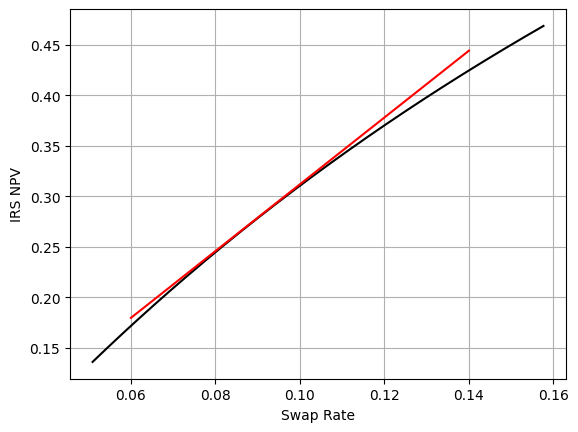
\includegraphics[width=0.8\linewidth]{dv01}
	\end{columns}
	\vspace{0.2cm}
\small{
	\item \emph{Positive convexity - receiving fixed}: as rates fall, the Swap price increases more than proportionally, amplifying your gains, but rising rates cause larger than expected losses.
	\item \emph{Negative convexity - paying fixed}: negative convexity exposes you to larger losses than expected when rates rise. Falling rates, however, benefit you less than proportionally.
	\item Longer-term Swaps generally have higher convexity (both positive and negative), meaning their prices are more sensitive to larger rate changes.
	\item Interest rate level: Convexity tends to be higher at lower interest rate levels because the price-yield curve is typically steeper in that range.}
\end{itemize}
\end{frame}

%\begin{frame}{Multiple Curve Bootstrapping}
%As mentioned above asset swaps are quoted as a spread to the swap curve. Recent market developments concerning yield curve construction, also known as bootstrapping, has lead to the introduction of multiple swap curves. This situation naturally led to the obvious question; which curve should asset swap spread benchmarked against? 
%After the credit crisis and the collapse of Lehman Brothers that followed in 2008 Libor rates, the rates at which banks lend to one another, were no longer considered risk-free. Interbank lending begain to incorporate credit risk and Libor rates began to price in, different levels of credit risk dependent on the loan term. The market standard 1M, 3M, 6M and 12M Libor rates started to reflect, for the first time, increasing levels of credit risk respectively as longer-term interbank lending became associated with greater credit risk.
%
%Furthermore, post credit crisis, tenor basis swaps began to quote with non-negligible spreads and as a result discounting and forecasting Libor rates from single yield curve was no longer viable. Yield curves were subsequently required to be built from tenor-homogenous instruments; that is instruments with the same coupon frequency and similar credit risk for consistency purposes.
%
%The market consequently adopted the overnight OIS rate as the risk-free discounting benchmark. This was because OIS swaps have a coupon frequency of 1 day, the shortest quoted frequency in the market, and market participants therefore adopted this rate to be the closest proxy to risk-free lending. In contrast however Libor forecasting needs to be derived from an appropriate Libor curve, namely the Libor curve calibrated with tenor homogeneous instruments i.e. instruments whose coupon frequency match the Libor rate to be forecasted. Typical market swap curves in this multi-curve regime are quoted with coupon frequencies of 1 day, 1
%month, 3 month, 6 month and 12 month and often referred to simply as an OIS, 1ML, 3ML, 6ML and 12L curve respectively, where the L denotes Libor.
%
%That is the term-structure of bond yields with the same issuer. Of course if there is short term distress in the market this might not be the case. A tenor basis swap is a swap is similar to a regular fixed-float swap, except that we have 2 floating legs with different floating rate frequencies e.g. 3M Libor vs 6M Libor.
%
%6.4 Benchmark Swap Curves
%Current EUR yield curves are charted below for reference in figure (14). The reader’s attention
%is drawn to the fact that EUR 1M and 3M Libor forward rates are negative on the short end of
%the curve. OIS rates are also negative in this region and the corresponding discount factors are
%greater than 1.0, which might have been considered unusual in previous years.
%A EUR swap is quoted as an annual fixed rate versus a semi-annual 6M Euribor rate as standard.
%Consequently the EUR benchmark swap curve has a floating frequency of 6 months. EUR asset
%swap spreads should be considered relative to the 6M Euribor curve. USD swaps are quoted
%semi-annual fixed versus 3M USD Libor, so the USD benchmark is the 3M Libor curve. This
%indicates that some basic familiarity with swap conventions is required to know which swap
%curve an asset swap spread is being quoted and benchmarked against.
%
%6.5 Curve Risk
%In an upward sloping yield curve environment, a high coupon bond normally has a lower modified duration than a low coupon bond. For example consider and compare the 1 5/8% 5/2026
%and 6% 6/2026 US Treasuries. The low coupon bond has a modified duration of 9.122 and the
%high coupon bond 7.697.
%If the yield curve steepens we expect the yield to rise further on the low coupon bond relative to
%the high coupon bond. Hence selling the low coupon bond and buying the high coupon bond in
%duration-neutral matched amounts will leave us with a steepening exposure in much the same
%way as if we were to buy an 8-year bond and sell a 10-year bond. This steepening exposure we
%call curve risk. Curve risk often manifests when trading asset swaps on a Yield-Yield basis since the duration of the swap is typically not identical to that of the offsetting bond.

%\begin{frame}{Swap Delta Measures}
%	\begin{itemize}
%		\item \textbf{Basis Point Value:} the variation (in EUR) of the swap $NPV$ in response to a 1 bp change in yields all along the yield curve (parallel shift in the yield curve). It is equal to the discounted value of the cash-flows for a rate of 0.01\% for all periods of the fixed leg with a rate of 0.01
%		\begin{equation}
%			BPV(t,T_\beta) = 0.01\%\sum_{i=\alpha+1}^{\beta}\tau_iP(0,T_i);
%		\end{equation}
%		\item \textbf{Modified Duration:} is the relative variation of a bond price given the variation of the reference rate. Since swaps can be thought of exchange of two bonds it can be used as a delta measure as well.
%	\end{itemize}
%	\begin{tikzpicture}[remember picture,overlay]
%	\node[xshift=5cm,yshift=-3.7cm] (image) at (current page.center) {
\includegraphics[width=20px]{python_logo}};
%	\node[align = center, yshift=1.45cm, below=of image] {\tiny{\href{shorturl.at/mqvFP}{shorturl.at/mqvFP}}};
%\end{tikzpicture}
%\end{frame}

%https://quant.stackexchange.com/questions/49582/interest-rate-swap-pv01-vs-dv01
%https://quant.stackexchange.com/questions/70346/fixed-vs-float-swap-interest-rate-risk/70426#70426
%https://math.nyu.edu/~avellane/DerivativeSecurities7.pdf

%1) Why does an interest rate swap have no duration, but it does have a DV01?
%
%Every spread product has duration and DV01 since all are sensitive to underlying moves in rates. To calc duration on a swap it's your notional/DV01 * 10k. As your swap reaches maturity the duration and DV01 factors down. Longer duration swaps, say 10Y vs 2Y, will inherently have more duration. Ex. a 10Y swap will have a duration slightly less than 10 depending on how much time to maturity left on the position.  
%
%For 2 and 3, do not think of each leg of the swap having DV01. Rather, the entire swap itself (both legs) is one position with DV01 depending on if you are paying/receiving fixed vs float.
%
%2) What does it mean for the fixed leg of an interest rate swap to have positive DV01?
%
%If you pay fixed and receive float, the entire swap has a positive DV01. Rates sell off (go higher), and you receive positive PnL on the position = positive DV01.
%
%3) Similarly, why does the floating leg of a swap have negative DV01, but contributes to positive DV01 since investor is paying floating?
%
%If you are paying floating and receiving fixed, the DV01 is negative since as rates go higher you need to pay out a higher amount which results in negative PnL on the position and thus negative DV01.


%\begin{frame}{Considerations}
%	\begin{itemize}
%		\item Higher rates affect the $NPV$ in two ways: via the discounting and via the forecasting. If the rates go higher the present value of both legs is lower, but the forecasted value of the floating leg is higher: forward rates are higher.
%		\item The way the curve is bootstrapped interferes with the calculation of the delta also for bullet swaps especially in the front end because the curve is bootstrapped using different instruments.
%	\end{itemize}
%\end{frame}

\begin{frame}{Trading and Hedging Swaps}
	\begin{itemize}
		\item With a Swap you can have a clear picture of the market. For example if you own the $5y$, you make money if rates go higher, loose money if they go lower.
		\item With two Swaps instead you can bet on the \textcolor{red}{slope} of the interest rate curve.
		\item If you bet on steepening of the $30y-10y$ slope, you pay the $10y-30y$; if you bet on flattening on the same portion of the yield curve you receive the $10y-30y$.		
		\item With Swaps you can bet on the \emph{bund basis}: this quantity is linked to the evolution of credit and liquidity in the inter-bank and Government bond markets.
	\end{itemize}
\end{frame}

%%\begin{frame}{Trading and Hedging Swaps}
%%	For example, the yield spread is 0.6524\%. An investor believes that this yield spread will narrow as inter-bank credit improves relative to German Sovereign credit. By entering into a position which profits from a rise in the lower (German	Sovereign) yields and / or a fall in the higher (inter-bank) yields, the investor is able to express his view on relative credit pricing.
%%	AGGIUNGERE UN PO' DI SPIEGAZIONE
%%\end{frame}

\begin{frame}{Homework}
\begin{itemize}
\item Ex.1
\end{itemize}
\end{frame}

\section{Cap and Floor}
\begin{frame}{Caps and Floors}
	\begin{itemize}
		\item<1-> A \textcolor{red}{Cap} is a Payer IRS in which the payment is done only if the payoff is positive. Its value is the expectation of 
		\begin{equation}
			\sum_{i=\alpha+1}^{\beta}D(t,T_i)N\tau_i\max\left[L(T_{i-1},T_i)-K,0\right]
			\label{eq:cap}
		\end{equation} 
		\item<2-> The cap allows investors which have a debt at a variable rate to buy insurance against high rates in the future.
		\item<3-> A \textcolor{red}{Floor} is the same kind of object but analogous to a Receiver IRS:
		\begin{equation}
			\sum_{i=\alpha+1}^{\beta}D(t,T_i)N\tau_i\max\left[K-L(T_{i-1},T_i),0\right]
			\label{eq:floor}
		\end{equation} 
	\end{itemize}
\end{frame}

\subsection{Caplets}
\begin{frame}{Caplet and Floorlet}
	\begin{itemize}
		\item<1-> Considering each element of the sum in \cref{eq:cap} or \cref{eq:floor} we see that Cap/Floor can be split into forward starting options over a floating rate, called \textcolor{red}{Caplet/Floorlet}.
		\item<2-> A Caplet/Floorlet payoff is defined as
		\begin{equation*}
			D(t,T_i)N\tau_i\max\left[L(T_{i-1},T_i)-K,0\right]
		\end{equation*} 
		and its value is given by
		\begin{equation}
			\textbf{Cpl}(t,T_{i-1},T_i,\tau,N,K)=\expect{Q}\left[e^{-\int_t^{T_i}r_s ds}N\tau(L(T_{i-1},T_i)-K)^+ | \mathcal{F}_t\right]
		\end{equation}
		\item<3-> This can also be written
		\begin{equation*}
			\textbf{Cpl}=N\expect{Q}\left[e^{-\int_t^{T_{i-1}}r_s ds}\tau P(T_{i-1},T_i)(L(T_{i-1},T_i)-K)^+ | \mathcal{F}_t\right]
		\end{equation*}
	\end{itemize}
\end{frame}

\begin{frame}{Caplets as ZCB Put Options}
	\begin{itemize}
		\item<1-> Using the LIBOR rate definition we get
		\begin{equation*}
			\begin{aligned}
				\textbf{Cpl} &=N\expect{Q}\left[e^{-\int_t^{T_{i-1}}r_s ds}P(T_{i-1},T_i)\left(\frac{1}{P(T_{i-1},T_i)}-1-K\tau\right)^+ \Big\rvert \mathcal{F}_t\right] \\
				& = N\expect{Q}\left[e^{-\int_t^{T_{i-1}}r_s ds}\left(1-(1+K\tau)P(T_{i-1},T_i)\right)^+ | \mathcal{F}_t\right]
			\end{aligned}
		\end{equation*}
		\item<2-> Multiplying by $\frac{1}{1+K\tau}$ we finally get
		\begin{equation}
			\textbf{Cpl}=N(1+K\tau)\expect{Q}\left[e^{-\int_t^{T_{i-1}}r_s ds}\left(\frac{1}{1+K\tau}-P(T_{i-1},T_i)\right)^+ \Big\rvert \mathcal{F}_t\right]
		\end{equation}
	\end{itemize}
	\only<3->{
	\begin{block}{Intepretation}
	Caplets can be seen as \textcolor{red}{put options} on ZCBs. Similarly floorlets are \textcolor{red}{call options} on ZCBs.
	\end{block}}
\end{frame}

\section{The Black Model}
\begin{frame}{The Black Model - Overview}
	\begin{itemize}
		\item The \textcolor{red}{Black Model} extends the Black-Scholes formula to \emph{caplets}, \emph{swaptions} and \emph{bond options}. %It uses the forward coordinates, not the spot ones; this last is not a minor issue indeed.
		\item The main difference with respect to the Black-Scholes set up is that \textcolor{red}{forward rates (or swap rates...) are log-normally distributed}, rather than the spot price of the underlying.
		\item So $F(t;T_{i-1},T_i)$ (or $S_\alpha(t)$) are modeled as log-normal random variables. 
		\item\textcolor{red}{But not at the same time !} 
		\item If $F(t;T_{i-1},T_i)$ is log-normal, then $S_\alpha(t)$ cannot be.
		\item \textcolor{red}{A single model cannot do the job.}
	\end{itemize}
\end{frame}

%\begin{frame}{The Black Model: Overview}
%	\begin{itemize}
	%		\item It should be recognized that the Black model is being actually used in different ways. In particular the caps uses the forward short-term LIBOR rate as the underlying state variable, whereas the swaptions uses longer-term forward swap rates. Beause forward swap rates are nearly linera in individual forward rates , the lognormality assumption implicit in the Black model cannot hold simultaneously for both, since a linear combination of lognormal variables is not lognormal.
	%	\end{itemize}
%\end{frame}

\begin{frame}{The Black Model: Overview}
	\begin{itemize}
		\item It is widely used in practice. 
		\item Black formula was indeed the metric by which traders translated volatilities into prices until rates became too low and the model collapsed under the assumption of positive rates.
		\item ...but for the moment we cannot consider it as a model ! Just a bunch of formulas.
		
		Their formal justification will be provided later in the context of the \textcolor{red}{Libor Market Model}.
	\end{itemize}
\end{frame}

\begin{frame}{Pricing Caps with the Black-76 Formula}
	\begin{block}{Definition}
	\begin{equation}
		\begin{aligned}
		\textbf{Cap}_{Bl}(0, \tau,N,K,\sigma_{\alpha,\beta}) &= N\sum_{i=\alpha+1}^{\beta}\textbf{Caplet}_{Bl}(T_i, \tau,K,\sigma_{\alpha,\beta}) = \\ &=N\sum_{i=\alpha+1}^{\beta}\tau P(0,T_i) \textbf{Bl}(K,F(0;T_{i-1},T_i),v_i)
		\end{aligned}
		\label{eq:cap_black}
	\end{equation}
	where
	\begin{equation*}
		\begin{gathered}
			\textbf{Bl}(K,F_i,v_i)=F\Phi(d_1(K,F_i,v_i)) - K\Phi(d_2(K,F_i,v_i)) \\
			d_{1,2} = \frac{\log{\cfrac{F_i}{K}} \pm \cfrac{v_i^2}{2}}{2} \\[0.2cm]
			v_i = \sigma_{\alpha,\beta}\sqrt{T_{i-1}}	
		\end{gathered}
	\end{equation*}
	\end{block}
\end{frame}

\begin{frame}{Problems with the Black Model}
\begin{itemize}
	\item In the Black model \textcolor{red}{negative rates are not allowed}. Hence a zero strike floor cannot be priced
	\begin{equation*}
		d_{1,2} = \frac{\boxed{\log{\frac{F}{K}}} \pm \cfrac{v^2}{2}}{2} 
	\end{equation*}
	but in the last years in the inter-bank market it was not so unusual to find prices for -1\% strike floors.
	\item Moreover in the Black model the empirical evidence of the "smile" (volatility vs $K$) is not accounted for, i.e. $\sigma$ is a constant. Two caps identical but for the strike need a different volatility to recover two different market prices if one uses Black formula.
	%\item And this is clear if one looks at the distribution and at the process of $F(t, T, S)$; the volatility does not depend on the strike of the option. It is a characteristic of the forward rate.
\end{itemize}
\end{frame}

\begin{frame}{The Practitioner Solutions}
\begin{itemize}
	\item \textbf{"Smile" issue}: the model is used with \textcolor{red}{different input volatilities for different strikes}. In practice it is a mapping of implied volatilities into prices and vice versa.
	\item \textbf{Non-positive rates}: could have switched to a different dynamics, like ABM, where negative values are "normal". But there are large differences in the tails between normal and log-normal distributions.
	So Black model has been \textcolor{red}{shifted}. The technique was already known but in the last years has become crucial to shift the lower bound of prices admitted by the model.
\end{itemize}
\end{frame}

\begin{frame}{Shifted Log-normal Model for Caplets}
\begin{itemize}
	\item It can be shown that Black formula provides valid solutions if strike and forward rate are \textcolor{red}{shifted}. For a $(T,S)$ caplet with strike $K$ we get
	\begin{equation}
		\textbf{Caplet}_{Bl}(t,T,S,\tau,K,v_T,\alpha) = P(t,S) Bl(K+\alpha,F(t;T,S)+\alpha,v_T)
	\end{equation}
	where $d_1$ and $d_2$ read as before and instead $v_i$ is now given by
	\begin{equation*}
		v_i = \sigma^{\text{shifted}}\sqrt{T_{i-1}}
	\end{equation*}
	\item The market quotes of $\sigma^{\text{shifted}}$ refer to shifts $\alpha$ of the order of [2\%,3\%].
	%\item What is the relationship between $\sigma^{\text{shifted}}$ and $v_T$ ?
	%\item Rewrite the Black-76 SDE for the $(T, S)$ caplet as follows
	%\begin{equation}
	%	dF(t,T,S)=\sigma^{\text{shifted}}(F(t,T,S)-\alpha)dW^{\mathcal{Q}_S}(t)
	%\end{equation}
	%\item It is easy to see that the price for a $(T,S)$ caplet with strike $K$ is given by
	%\begin{equation}
	%	Cpl(t,T,S,\tau,K,v_T,\alpha)=P(t,S)Bl(K-\alpha,F(t,T,S)-\alpha,v_T)
	%\end{equation}
\end{itemize}
\end{frame}

\subsection{Cap/Floor Volatility}
\begin{frame}{Flat Volatilities}
	\begin{itemize}
		\item When comparing to other vanilla derivatives, Cap/Floor pricing offers an additional complexity, as it does not involve a single volatility number. 
		\item As seen Cap/Floor can be \textcolor{red}{stripped} into Caplet/Floorlet which should be priced with a different volatility each. 
		\item However, in the market, \textbf{Cap} quotes are computed according to the following 
		\begin{equation*}
			\textbf{Cap}(0,\mathcal{T}_j,K)=N\sum_{i=1}^{j}\tau P(0,T_i) \textbf{Bl}(K,F_i(0),v_{\mathcal{T}_j}^{cap})
		\end{equation*}
		where the same "average" volatility value $v_{\mathcal{T}_j}^{cap}$ is used in each caplet. 
		\item $v_{\mathcal{T}_j}^{cap}$ is called \textcolor{red}{flat volatility}, and is typically quoted for a range of strikes and expiries over liquid floating rates (e.g. 3M and 6M Euribor).
	\end{itemize}
\end{frame}

\begin{frame}{Spot Volatilities}
	\begin{itemize}
		\item Notice that the same average volatility $v_{\mathcal{T}_j}^{cap}$ is assumed for all caplets in the $T_j$-maturity cap. 
		%\item However, when the same caplets concur to a different cap, say a $T_{j+1}$-maturity cap, their average volatility is changed. 
		\item This appears to be somehow inconsistent. In the cap volatility system, the same caplet is linked to different volatilities when concurring to different caps.
		\item The correct volatilities can be recovered with a numerical procedure (i.e. \emph{bootstrapping}) from
		\begin{equation*}
		\sum_{i=1}^{j}\tau P(0,T_i) \textbf{Bl}(K,F_i(0),v_{\mathcal{T}_j}^{cap}) = \sum_{i=1}^{j}\tau P(0,T_i) \textbf{Bl}(K,F_i(0),v_{\mathcal{T}_{i-1}}^{caplet})
		\end{equation*}
		\item $v_{\mathcal{T}_{i-1}}^{caplet}$ are called \textcolor{red}{spot volatilities} (different $v_{\mathcal{T}_{i-1}}^{caplet}$ are assumed for different caplets concurring to the $Tj$-maturity cap).
		\item Although being quoted, \textcolor{red}{flat volatilities have little financial meaning}. Conversely spot volatilities cannot be observed directly but are the quantities \textcolor{red}{naturally tied to forward rates as a measure of their uncertainty}.
	\end{itemize}
	\begin{tikzpicture}[remember picture,overlay]
	\node[xshift=5cm,yshift=-3.9cm] (image) at (current page.center) {
\includegraphics[width=80px]{python}};
	\end{tikzpicture}
\end{frame}

%\begin{frame}{The Volatility Hump}
%\begin{itemize}
%	\item Empirical studies have pointed out two very important facts:
%	\begin{itemize}
%		\item the first one is that interest rates volatility can depend on the level of the interest rates themselves;
%		\item moreover the volatility function is increasing in the short end of the curve, and decreasing in the long end, with an \textcolor{red}{humped} type movement.
%	\end{itemize}  
%	\begin{columns}
%		\column{0.45\linewidth}
%		\item Uncertainty is bigger in the intermediate region and lower in the front of the maturity spectrum. For long maturities volatility tends to decay.
%		\item When the hump does not appear it is regarded as \emph{stressed market}.
%		%\item There is a financial explanation for this feature.
%		\column{0.45\linewidth}
%		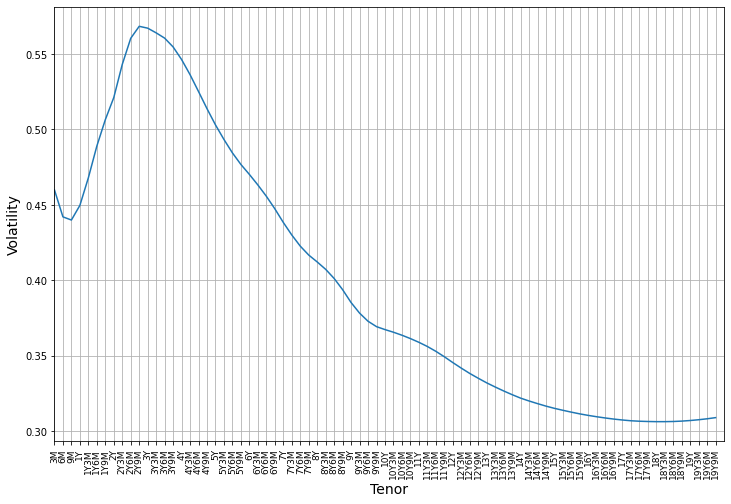
\includegraphics[width=1.1\linewidth]{cap_vola}
%	\end{columns}
%\end{itemize}
%\end{frame}

\section{Swaptions}
\begin{frame}{Swaptions Overview}
\begin{itemize}
	\item<1-> The purchaser of an \textcolor{red}{European swaption} has the right but not the obligation to enter into a swap contract, at a given future time, called the \textcolor{red}{swaption maturity}.
	\item<2-> There are two types of \textcolor{red}{swaptions} (as the underlying swaps): a \emph{payer} in which at maturity the buyer could become the fixed-rate payer and a \emph{receiver} where she could become the fixed-rate receiver.
	\item<3-> A swaption provides protection for a borrower as it ensures a maximum fixed interest rate payable in the future. Furthermore, it gives her the flexibility, if the rate does not rise above the swaption strike rate at expiry, to choose not to exercise it and take advantage of the lower market rates.
\end{itemize}
\end{frame}

\begin{frame}{Swaptions Overview}
	\begin{itemize}
	\item<1-> Usually, the swaption maturity coincides with the first reset date of the underlying IRS (the Interest Rate Swap length is called the \textcolor{red}{tenor} of the swaption).	
	\item<2-> If you are on the buyer side (you are long payer swaption) which is your view on rates ? Why ?
	\item<3-> Are there any risks associated with a Swaption?
	\begin{itemize}
		\item<4-> The primary risk with a Swaption occurs after you have exercised your right and proceeded with the Swap. Should interest rate movements be different to your expectations, the Swap may have the opposite effect to what you were trying to achieve with the transaction. 
		\item<5-> If interest rates do not rise above the strike on the exercise date, you have not obtained any benefit from the premium paid for the purchase of the Swaption. The premium is the cost of obtaining protection against a rise in interest rates.
	\end{itemize}
\end{itemize}
\end{frame}

\begin{frame}{Swaption Payoff}
\begin{itemize}
	\item<1-> The discounted payoff of a payer Swaption (with maturity $T_\alpha$) is given, recalling the value of a payer IRS (\cref{eq:swap_as_sum_fra}) by
	\begin{equation}
		\textbf{PSw}=D(t,T_\alpha)\left(\sum_{i=\alpha+1}^\beta P(T_\alpha,T_i)\tau_i (F(T_\alpha;T_{i-1},T_i) - K)\right)^+
		\label{eq:swaption_payoff_std}
	\end{equation}
	\item<2-> Unfortunately this payoff \textcolor{red}{cannot} be easily decomposed into elementary parts (as done for Cap/Floor). Indeed the \emph{positive part operator} $(\cdot)^+$ is "outside" the summation (while for Caps it is "inside").
	\item<3-> Nevertheless it can be simplified by writing it in a different way...
	%		\begin{equation}
		%			ND(t,T_\alpha)\left(S_{\alpha,\beta}(T_\alpha)-K\right)^+\sum_{i=\alpha+1}^\beta \tau_i P(t,T_i)
		%		\end{equation}
\end{itemize}
\end{frame}

\begin{frame}{Swaption Payoff}
\begin{itemize}
	\item<1-> Recall that we have expressed the swap payoff also as (\cref{eq:swap_payoff_with_swap_rate})
	\begin{equation*}
	\textbf{PFS}=\sum_{i=\alpha+1}^\beta \tau_i P(t,T_i)(S_{\alpha,\beta}-K) = A(S_{\alpha,\beta}-K)
	\end{equation*}
	\item<2-> If we look at the swaption payoff through this expression modeling as stochastic variable directly $S_{\alpha,\beta}(t)$, instead of each forward rate $F(t;T_{i-1},T_i)$, we can write the swaption price as the expectation of
	\begin{equation}
		\textbf{PSw}=\expect{Q}\left[D(t,T_\alpha)A\max(S_{\alpha,\beta}(T_\alpha)-K, 0)\right]
	\end{equation}
	which looks like easier and more intuitive than previous \cref{eq:swaption_payoff_std}.
\end{itemize}
\end{frame}

\begin{frame}{Swaption Characterization}
	\begin{itemize}	
		\item We characterize the payoff in three different ways
		\begin{enumerate}
			\item The swaption is said to be \textcolor{red}{at-the-money} (ATM) if
			\begin{equation*}
				K = K_{ATM} = S_{\alpha,\beta}(0) = \frac{P(0,T_\alpha)-P(0,T_\beta)}{\sum_{i=\alpha+1}^\beta \tau_i P(0,T_i)}
			\end{equation*}
			where $T_\alpha$ is the maturity of the swaption, and $T_\beta$ the last payment date of the underlying swap (the first being $T_{\alpha+1})$. That is when the strike is equal to the swap forward rate $S_{\alpha,\beta}$.
			\item The payer swaption is \textcolor{red}{in-the-money} if $K<K_{ATM}$ and \textcolor{red}{out-of-the-money} otherwise.
			\item The opposite holds for the receiver swaption.
		\end{enumerate}
		\item ATM swaptions are quoted for maturities ranging between $1m$ and $30y$, and for tenors between $1y$ and $30y$.
	\end{itemize}
\end{frame}

%\begin{frame}{Swaption as an Option on a Swap}
%	\begin{itemize}
%		\item So the forward rates are the chosen state variable, also the correlation between them is needed...
%		\item Market practice: approximation formula (see chapter 6 of Brigo-Mercurio) the definitive reference for this issue.
%		\item Clearly here a model which accounts for terminal correlations needed.
%		\item Which is the relationship between a Cap and a payer swaption with the same payment and roll dates ?
%	\end{itemize}
%
%\end{frame}

\begin{frame}{An Example}
	\begin{itemize}
		\item \textbf{A} has raised a $10y$ loan with floating interest rates fixed every three months (IBOR + margin).
		\item \textbf{A} wants to \emph{hedge the loan against rising interest rates but also to benefit from the floating rate}, i.e. should interest rates not rise above a certain level (the swaptions strike-rate $K$).
		\item The purchase of a payer swaption could hedge this risk: 
		\begin{columns}
			\column{0.45\linewidth}
			\begin{itemize}
				\item \textbf{interest rates increase}: \textbf{A} may exercise the swaption and be a party of a swap as a payer of a fixed interest rate;
				\item \textbf{swap-rate below $K$}: it will not be exercised and \textbf{A} will continue to have floating-rate funding.
			\end{itemize}
			\column{0.45\linewidth}
			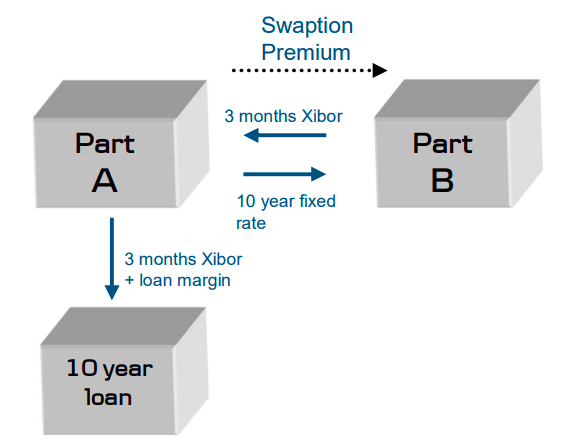
\includegraphics[width=1.\linewidth]{swaption_example}
		\end{columns}
	\end{itemize}
\end{frame}

\begin{frame}{Homework}
\begin{itemize}
\item In order to hedge your position against interest rate movements which kind of contract would you use: 
\begin{itemize}
\item a Swap
\item a Cap/Floor
\item a Swaption
\end{itemize}
List the pros and cons about each one and declare your favourite.
\end{itemize}
\end{frame}

\begin{frame}{Differences between Caps and Swaptions}
\begin{itemize}
	\item<1-> Caps can be decomposed into more elementary products: \textcolor{red}{caplets}. Value each caplet one by one and then add their prices
	\begin{itemize}
		\item each forward rate can be modeled as a random variable;
		\item \textbf{no joint action of forward LIBOR rates is involved.}
	\end{itemize}
	\item<2-> Unfortunately this is not possible with swaptions. The swap rate is \textcolor{red}{essentially a weighted average of forward rates} $S=\cfrac{\sum F(t;T_{i-1},T_i)}{\sum P(t,T_i)}$, hence its volatility should depend on each forward rate volatilities \textbf{as well as} their correlations.
	\item<3-> If you take as "fundamental" entity the LIBOR rates you have to deal with the joint action of the simple forward LIBOR rates and so with the \textbf{terminal correlation} between rates of different portions of the yield curve. 
	\item<4-> This issue will be extensively studied in the context of the Libor Market Models further on down the course.
	%Can you provide an example ?
\end{itemize}
\end{frame}

\subsection{Bond Options}
\begin{frame}{An Option to Exchange Fixed with Float}
\begin{itemize}
	\item<1-> We have seen that a Swap can be viewed as an exchange of bonds (fixed for float).
	\item<2-> Hence a Swaption can be regarded as an \textcolor{red}{option to exchange fixed for floating} bonds (or vice versa).
	\item<3-> To fully characterize this point we need an expression for a \textcolor{red}{Coupon Bond Option}.
	\item <4-> Most \emph{short rate models} have a closed formula for the Zero Coupon Bond price. It would be even simpler if we could express a Coupon Bond Option as a portfolio of Zero Coupon Bond Options.
	\item<5-> Luckily we can do that thanks to a recipe known as \textcolor{red}{Jamshidian's decomposition}.
\end{itemize}
\end{frame}

\begin{frame}{Jamshidian's Decomposition}
\begin{block}{Theorem}
	Consider a sequence of functions $f_i$, a random variable $W$ and a constant $K\ge0$. If each $f_i$ is monotone (decreasing), that is $\cfrac{\partial f_i}{\partial W} < 0;\;\forall i$, then 
	\begin{equation*}
		\left(K - \sum_i f_i(W)\right)^+ = 	\sum_i \left(K_i - f_i(W)\right)^+
	\end{equation*} 
	In financial terms it means that the payoff of an option on a portfolio of assets can be expressed in terms of a portfolio of options on each asset.
\end{block}
\end{frame}

\begin{frame}{Jamshidian's Decomposition Proof}
\begin{itemize}
	\item<1-> Since each $f_i$ is monotone also $\sum_i f_i$ is decreasing. Hence there is a unique solution $\hat{w}$ to 
	\begin{equation*}
		\sum_i f_i(\hat{w}) = K
	\end{equation*}
	\item<2-> Each $f_i$ is decreasing so
	\begin{columns}
	\column{0.7\linewidth}
	\uncover<2->{\begin{equation*}
	\left(K - \sum_i f_i(W)\right)^+ = \left(\sum_i f_i(\hat{w}) -  \sum_i f_i(W)\right)^+ = 
	\end{equation*}}
	\uncover<3->{\begin{equation*}
	= \left(\sum_i (f_i(\hat{w}) -  f_i(W))\right)^+= \sum_i (f_i(\hat{w}) - f_i(W))\mathbb{1}_{W\ge \hat{w}}
	\end{equation*}}
	\uncover<4->{\begin{equation*}
	= \sum_i \left(K_i - f_i(W)\right)^+
	\end{equation*}
	\myendproof
	}
	\column{0.35\linewidth}
	\uncover<1->{
	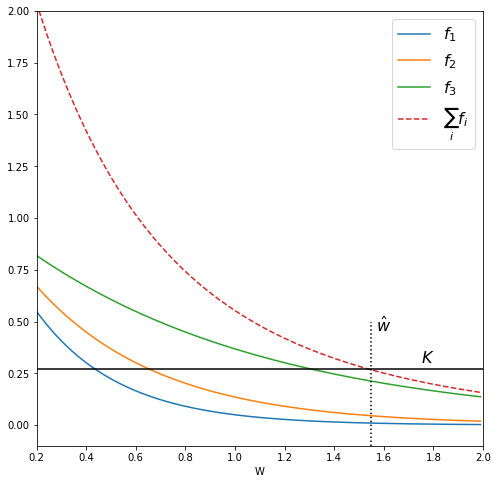
\includegraphics[width=1\linewidth]{jamshidian_trick}}
	\end{columns}
\end{itemize}
\end{frame}

\begin{frame}{Back to Coupon Bond Option}
\begin{itemize}
	\item<1-> Consider a coupon bond which pays the following cash flows $\mathcal{C}=\{c_1,\dots,c_n\}$ at dates $\mathcal{T}=\{T_1,\ldots,T_n\}$.
	\item<2-> Let $t\leq T_1$, the bond price is given by
	\begin{equation*}
		\textbf{CB}(t,\mathcal{C},\mathcal{T})=\sum_{i=1}^n c_i \Pi(t, T_i, r(t))
	\end{equation*}
	\item<3-> Suppose we would like to calculate the price of a put option with strike $K$ on this coupon bond. The payoff reads
	\begin{equation*}
		\textbf{CBP}=\left[K-\textbf{CB}(t,\mathcal{C},\mathcal{T})\right]^+ = \left[K-\sum_{i=1}^n c_i \Pi(t, T_i, r(t))\right]^+
	\end{equation*}
\end{itemize}
\end{frame}

\begin{frame}{Coupon Bond Option}
\begin{itemize}
	\item<1-> Now apply the Jamshidian's decomposition to previous payoff.
	\item<2-> First need to find the interest rate value $r^*$ such that $\sum_{i=1}^n c_i \Pi(t, T_i, r^*) = K$.
	\item<3-> Assuming the interest rate model satisfies the required condition
	\begin{equation*}
		\frac{\partial \Pi(t,T_i,r(t))}{\partial r}<0,\;\forall 0<t<s
	\end{equation*}
	we can rewrite the payoff as
	\begin{equation}
		\textbf{CBP}(t,T_i,\Pi,r^*) = \sum_{i=1}^n c_i [\Pi(t, T_i, r^*)-\Pi(t, T_i, r(t))]^+
	\label{eq:bond_option_payoff}
	\end{equation}
\end{itemize}
\end{frame}

\begin{frame}{Coupon Bond Option}
\begin{itemize}
	\item \cref{eq:bond_option_payoff} tells us that we can price a coupon bond option as a portfolio of options on ZCBs.
	\item The strike of these option is calculated as the value of a ZCB given a \emph{particular} value of the short rate, determined with a root finding procedure.
	\item In formulas the CBO with maturity $T$ and strike $K$ reads
	\begin{equation}
		\textbf{CBP}(t,\mathcal{T},\mathcal{C},K) = \sum_{i=1}^n c_i \textbf{ZBP}(t,T_i,\Pi,r^*)
	\end{equation}
\end{itemize}
\end{frame}

\begin{frame}{Adapting to Swaptions}
\begin{itemize}
	\item When interest rates are modeled using \textcolor{red}{Affine Short Rate Models} it is rather simple to arrive to the swaption pricing formula.
	\item \emph{Affine Models} indeed relates ZCB price to a spot rate model according to 
	\begin{equation*}
		P(t,T) = A(t,T)e^{-B(t,T)r}
	\end{equation*} 
	\item Hence the value $r^*$ can be determined as a solution of 
	\begin{equation*}
		\sum_{i=1}^n A(t,t_i)e^{-B(t,t_i)r^*}
	\end{equation*}		
	%%		\item Denote as usual with $\tau_i$ the year fraction between $t_{i-1}$ and $t_i$, fix $c_i=X\tau_i$ and $c_n = 1+X\tau_i$.
	%%		\item Let the swap notional be equal to N.
	%%		\item Thus for the price of a payer swaption we have to calculate the following payoff
	%%		\begin{equation*}
		%%			\left[1-CB(t,\mathcal{C},T)\right]^+
		%%		\end{equation*}
	%%		\item We can calculate this payoff via the procedure outlined before.
\end{itemize}
\end{frame}

\begin{frame}{Swaption Pricing via Affine Models}
\begin{itemize}
	\item Consider an option on a swap which pays a fixed rate $X$ and receives LIBOR.  
	\item Modeling the short rate with an affine model we can define $r^*$ at time $T$, such that
	\begin{equation*}
		\sum_{i=1}^n c_i A(t,T_i)e^{-B(t,T_i)r^*} = 1
	\end{equation*}
	where $c_i$ is the coupon value.
	\item Setting $X_i = A(t,T_i)e^{-B(t,T_i)r^*}$ the payer swaption price is thus given by
	\begin{equation}
		\textbf{PSw}(t,T,N) = N\sum_{i=1}^n c_i \textbf{ZBP}(t,T_i,X_i)
	\end{equation}
	while the receiver swaption price reads
	\begin{equation}
		\textbf{RSw}(t,T,N) = N\sum_{i=1}^n c_i \textbf{ZBC}(t,T_i,X_i)
	\end{equation}
\end{itemize}	
\begin{tikzpicture}[remember picture,overlay]
\node[xshift=6.0cm,yshift=-4.cm] (image) at (current page.center) {
\includegraphics[width=80px]{python}};
\end{tikzpicture}
\end{frame}

\begin{frame}{Black Formula for Swaptions}
\begin{itemize}
	\item Replacing the forward rate $F(0;t_{i-1},t_i)$ with the swap rate $S_{\alpha,\beta}(0)$ and plugging in the quoted swaption volatility you get Black's formula for swaptions
	\begin{equation}
		\begin{aligned}
			\textbf{PSw}_{Bl}(0,T,&N,K,S_{\alpha,\beta})=\\
			&N\left[S_{\alpha,\beta}(0)\Phi(d_1)-K\Phi(d_2)\right]\sum_{i=\alpha+1}^\beta P(0,T_i)\tau_i
		\end{aligned}	
	\end{equation}
	where
	\begin{equation*}
		d_{1,2} = \frac{\log{\frac{S_{\alpha,\beta}}{K}} \pm \frac{v^2}{2}}{2}
	\end{equation*}
	and
	\begin{equation*}
		v = \sigma_{\alpha,\beta}\sqrt{T_\alpha}
	\end{equation*}
\end{itemize}
\end{frame}

\begin{frame}{Swaptions Volatility Calibration}
\begin{itemize}
	\item Swaption volatilities are quoted for different maturities and tenors (length of the underlying swap).
	\item Both for ATM and away from ATM on both sides ("swaption smile").
	\item So swaptions have an additional dimension with respect to caps: the quotes are parametrized according to 
	\begin{itemize}
		\item maturites;
		\item tenors;
		\item strikes.
	\end{itemize}
	%\item They have also a different \emph{delta} effect on your book.
	%		\item Volatility trade between caps ans swaption: WEDGE
\end{itemize}
\end{frame}

\begin{frame}{Swaption Volatility Calibration}
  \begin{center}
    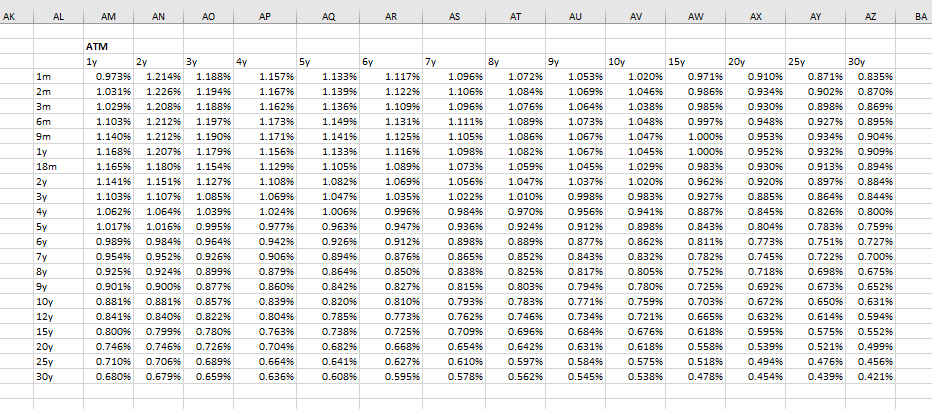
\includegraphics[width=1.\linewidth]{atm_vol}
  \end{center}
\end{frame}

\begin{frame}{Swaption Volatility Calibration}
  \begin{center}
    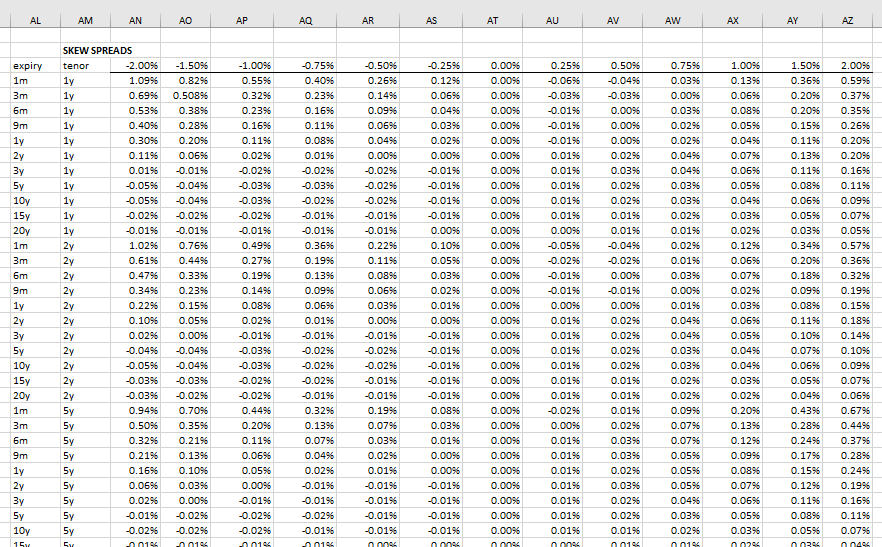
\includegraphics[width=1.\linewidth]{skews}
  \end{center}
\end{frame}

\begin{frame}{Swaption Volatility Calibration}
  After we have constructed the volatility matrix we can fit the ``smile'' at each (expiry, tenor) pair.

  This is done assuming the volatilities evolves according to the SABR model. An approximated solution has been given by \emph{Hagan et al.}
  \begin{eqnarray} \sigma _{B}(K,f) &=&\frac{\textcolor{red}{\alpha} \left\{ 1+\left[ \frac{\left( 1-\textcolor{red}{\beta} \right) ^{2}}{24}\frac{\textcolor{red}{\alpha} ^{2}}{(fK)^{1-\textcolor{red}{\beta}}}+\frac{1}{4}\frac{\textcolor{red}{\rho \beta \nu\alpha}}{(fK)^{(1-\textcolor{red}{\beta})/2}}+\frac{2-3\textcolor{red}{\rho} ^{2}}{24}\textcolor{red}{\nu}^{2}\right] T\right\} }{(fK)^{(1-\textcolor{red}{\beta})/2}\left[ 1+\frac{(1-\textcolor{red}{\beta})^{2}}{24}\ln ^{2} \frac{f}{K}+\frac{(1-\textcolor{red}{\beta})^{4}}{1920}\ln^{4}\frac{f}{K}\right] } \times \frac{z}{\chi (z)} \notag \\ z &=&\frac{\textcolor{red}{\nu}}{\textcolor{red}{\alpha}}(fK)^{(1-\textcolor{red}{\beta})/2}\ln \frac{f}{K} \notag \\ \chi (z) &=&\ln \left[ \frac{\sqrt{1-2\rho z+z^{2}}+z-\textcolor{red}{\rho}}{1-\textcolor{red}{\rho}}\right] . \notag \end{eqnarray}
\end{frame}

\begin{frame}{Swaption Volatility Calibration}
    \begin{center}
      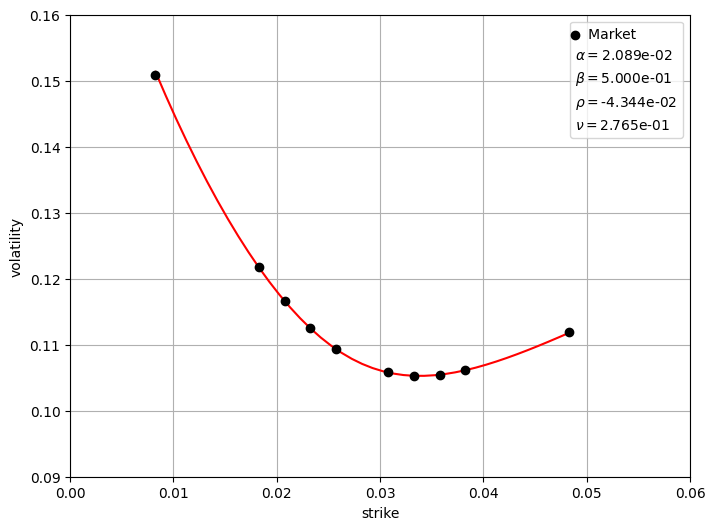
\includegraphics[width=0.65\linewidth]{10y_10y}
    \end{center}
\end{frame}

\begin{frame}{Swaption Volatility Calibration}
    \begin{center}
      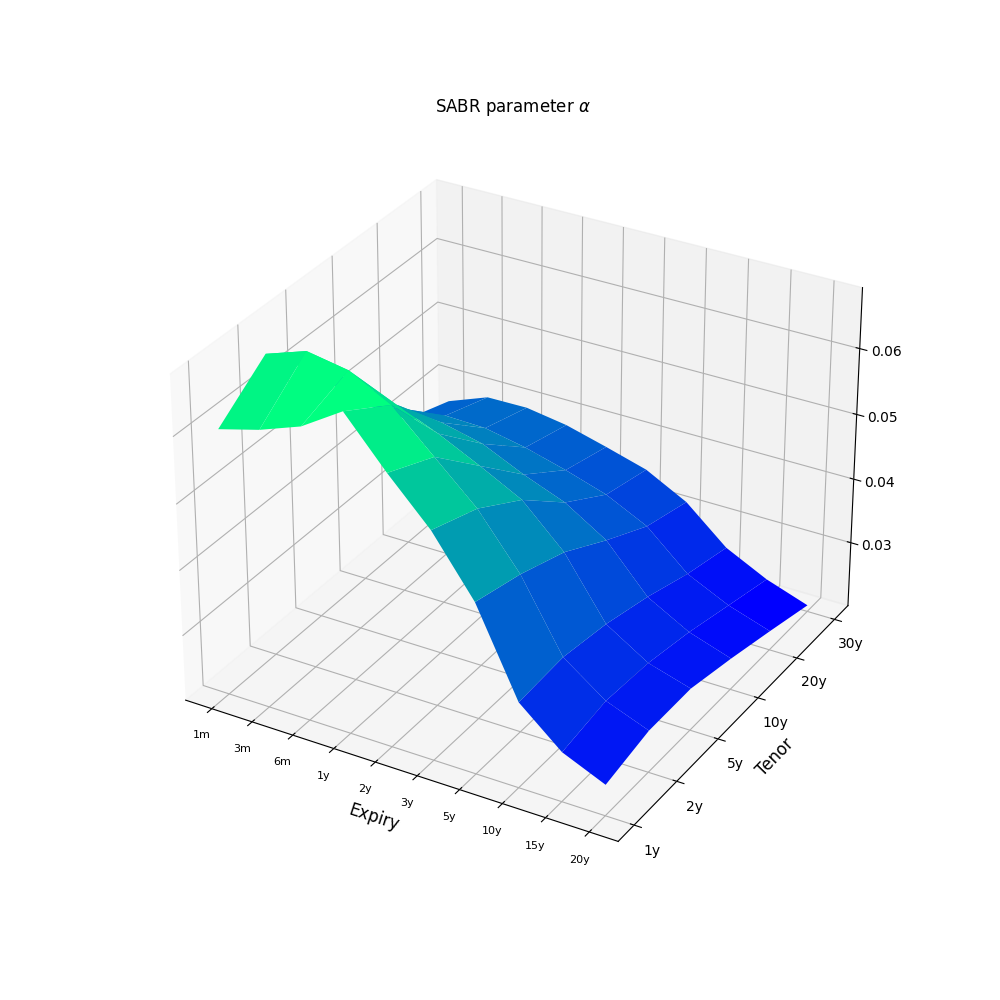
\includegraphics[width=0.3\linewidth]{alpha}
      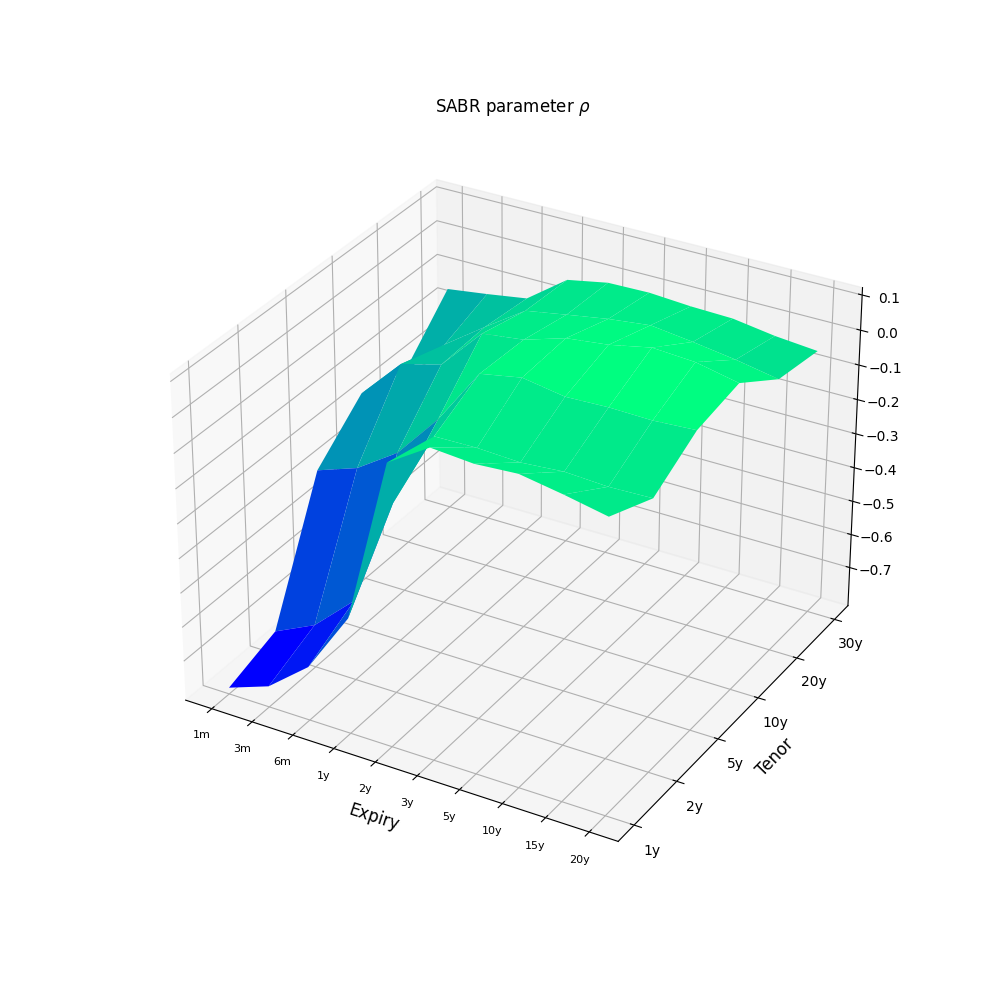
\includegraphics[width=0.3\linewidth]{rho}
      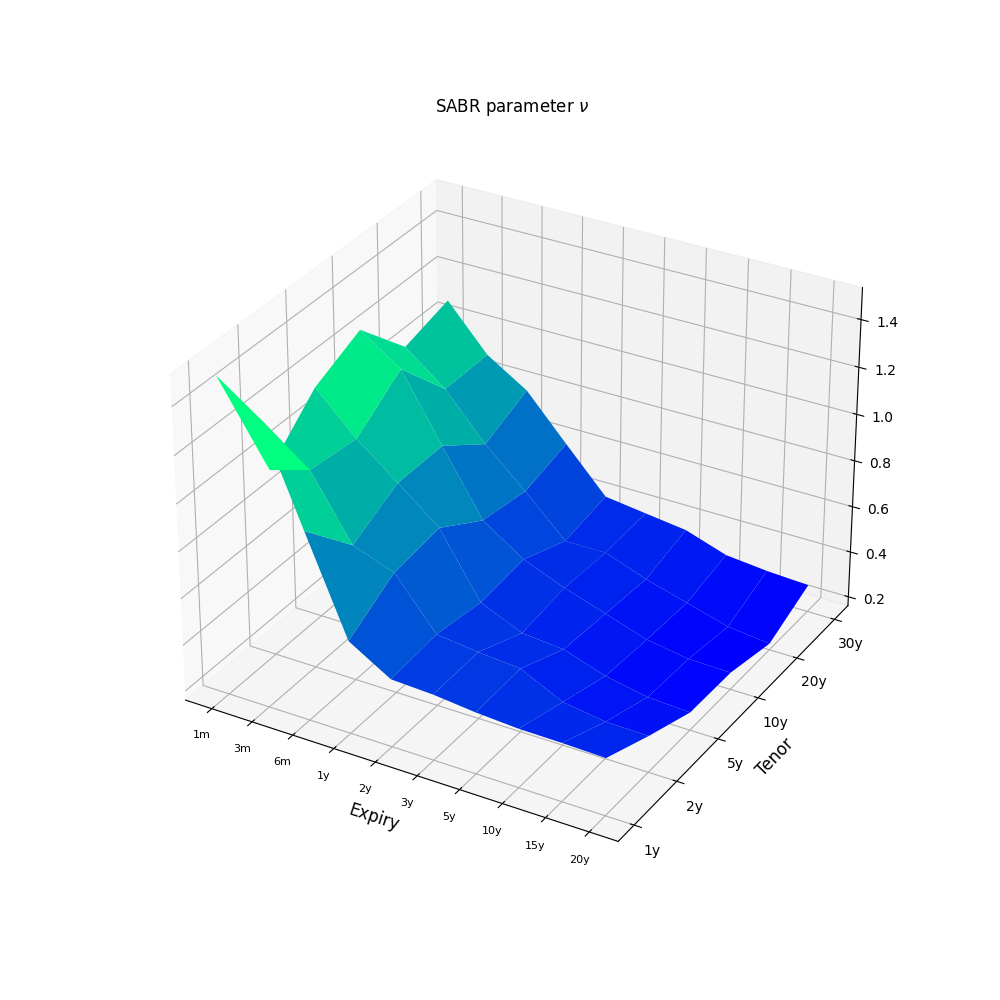
\includegraphics[width=0.3\linewidth]{nu}
    \end{center}
\end{frame}

\subsection{Bermudan Swaption}
\begin{frame}{Bermudan Swaptions}
\begin{itemize}
	\item<1-> It is a swaption in which the optionality can be exercised at a \textcolor{red}{predetermined set of dates} (not only one).
	\item<2-> It is useful for hedging callable bonds (especially if step-up, i.e. with the coupon increasing with time).
	\item<3-> A \textcolor{red}{Bermudan Swaption} gives the holder the right but not the obligation to enter in an interest rate swap contract at different dates (usually the swap reset dates) with some days of notification to the counter-party.
	\item<4-> The interest rate swap the holder can enter into, is the same existing contract, so if the holder does not exercise at the first date in the call schedule, the option for the following periods is written on shorter swaps.
\end{itemize}
\end{frame}

\begin{frame}{Bermudan Swaption Example}
\begin{itemize}
	\item<1-> As an example consider the following: receiver Bermudan Swaption written on a 3 years swap with the first call date $2y$ from now (we suppose semi-annual payments).
	\item<2-> If at the end of the second year she will not exercise, six months later she will have to decide if entering or not in the same remaining swap which now has become a $2y6m$ swap.
	\item<3-> If again she will not exercise the last possibility will involve the decision of whether or not to enter on the $2y6m-3y$~$FRA$.
\end{itemize}
\end{frame}		

%\begin{frame}{Bermudan Swaption Payoff}
%\begin{itemize}
%	\item At the maturity $T$, the payoff of a Bermudan swaption is given by
%	\begin{equation*}
%		\textbf{BS}(T) = \max(0, V_{\text{swap}}(T))
%	\end{equation*}
%	where $V_{swap}(T)$ is the value of the underlying swap in $T$.
%	\item At any exercise date $T_i$, the payoff of the Bermudan swaption is given by
%	\begin{equation*}
%	\textbf{BS}(T_i) = \max(K(T_i), V_{\text{swap}}(T_i))
%	\end{equation*}
%	where $V_{\text{swap}}(T_i)$ is the exercise value of the swap and $K(T_i)$ is the intrinsic value, i.e. the holder of the option receives $\max(K(T_i), 0)$ if the option is exercised at time $T_i$.
%	CONTROLLARE ULTIMO DISCORSO
%\end{itemize}
%\end{frame}

\begin{frame}{Bermudan Swaption Pricing}
\begin{itemize}
	\item<1-> Some interest rate instruments can be priced just looking at the term structure (FRA and Swaps)
	\begin{itemize}
		\item the only problem is: which is the right term structure ? (this is a lesson from the 2008 crisis).
	\end{itemize}
	\item<2-> Some other instruments cannot be priced only with the yield curve: we need the future (risk-neutral) evolution of the rates.
	%\item Non-linearities come in !
	%\item Swaptions are non-linear products and may require to model the correlation between forward LIBOR rates.
	\item<3-> Given the complexity of Bermudan swaption valuation, there is no closed form solution. Therefore, we need to select an interest rate term structure model and a numeric solution to price this contract numerically.		
	\item<4-> Typically tree techniques or the Longstaff-Schwartz method are used.
	\begin{tikzpicture}[remember picture,overlay]
		\node[xshift=5.8cm,yshift=-4.cm] (image) at (current page.center) {
\includegraphics[width=80px]{python}};
	\end{tikzpicture}
\end{itemize}
\end{frame}

%\begin{frame}{Bermudan Swaption Pricing: Outline}
%	\begin{itemize}
%	\item<1-> Consider a tenor structure $\mathcal{T}=\{T_i\}^\beta_{i=\alpha}$ and a Bermudan receiver swaption with time $t$ value $\textbf{RBS}(t,K)$.
%	\item<2-> Assuming no prior exercise, at any time point $T_i$ the swaption holder has the right to receive the exercise value $V_e$ of the swaption, i.e., present value of the underlying swap:
%	\begin{equation}
%	V_e(T_i)=(K-S_{i,\beta}(T_i))+\sum^\beta_{k=i+1} P(T_i,T_k)\tau_k
%	\label{eq:exercise_value}
%	\end{equation}
%	\item<3-> The exercise value has to be compared to the so-called continuation value, $V_c$, of holding the option beyond $T_i$:
%	\begin{equation}
%	V_c(T_i)=\mathbb{E}[\textbf{RBS}(T_{i+1},K)|S_{i,\beta}(T_i)]
%	\label{eq:continuation_value}
%	\end{equation}
%\end{itemize}
%\end{frame}
%
%\begin{frame}{Bermudan Swaption Pricing: Outline}
%	\begin{itemize}
%		\item<1-> The value of the Bermudan swaption can now be given in terms of \cref{eq:exercise_value} and \cref{eq:continuation_value}, recursively.
%		\item<2-> The evaluation of proceeds backward in time: at $T_{\beta-1}$
%		the value of the Bermudan is known, i.e. the swaption payoff
%		\begin{equation*}
%			\textbf{RBS}(T_{\beta-1},K)=P(T_{\beta-1},T_\beta)\tau_\beta(K-S_{\beta-1,\beta}(T_{\beta-1}))^+
%		\end{equation*}
%		\item <3->This allows to update the continuation value at $T_{\beta-2}$ with \cref{eq:continuation_value} and compare it to the exercise value
%		\begin{equation*}
%			\textbf{RBS}(T_j,K)=\max(V_e(T_j),V_c(T_j)),\quad\text{for }j=\beta-2,\beta-3,\ldots,n
%		\end{equation*}
%	\end{itemize}
%\end{frame}
%
%\begin{frame}{Bermudan Swaption Pricing: Outline}
%	\begin{itemize}
%		\item<1-> This procedure of comparing “backwardly-cumulated” continuation value with exercise value and deciding upon a swaption exercise is repeated until the initial valuation date is reached, at which point the algorithm yields a price estimate for the Bermudan swaption. 
%		\item<2-> The calculation of the continuation value is clearly model-dependent and the choice of modeling framework itself often determines the scope of available numerical techniques.
%\end{itemize}
%\end{frame}

\subsection{Callable Bonds}
\begin{frame}{Callable Coupon Bond}
\begin{itemize}
	\item<1-> A \textcolor{red}{callable bond} is a bond in which, on the call date(s) (there can be more than one), the issuer has the right, but not the obligation, to buy back (redeem) the bonds from the bond holders at a defined call price.
	\item<2-> We have seen that a swap can be regarded as an exchange of bonds. It is easy to guess that a replica for the callable bond price can be obtained by simply adding a (swap-)option to the swap used to price the underlying bond.
	\item<3-> If there are multiple callability dates is clear that the swaption we need is a Bermudan one.
	\item<4-> With a receiver bermudan swaption with the same contractual conventions of the Swap (i.e. the strike of the swaption is equal to the coupon of the bond) we can offset the swap. %; which represents the economic equivalent of calling the bond at par.
	%\item So $\max(CCBP(T,S,K,\tau)-100, 0)$ can be represented as $\max(K-S(T_j,\beta)(T), 0)$.
	%\item Intuition: long on the bond, short on the rates.
\end{itemize}
\end{frame}

\begin{frame}{Callable vs Non Callable Coupon Bonds}
\begin{itemize}
	\item<1-> \emph{Ceteris paribus} a non callable coupon bond has an higher price than a callable one because the callability option adds value to the issuer
	\begin{equation*}
		\text{price of callable bond} = \text{price of straight bond} – \text{price of call option}.
	\end{equation*}
	\item<2-> If interest rates decline, the issuer of a callable bond can issue new debt, receiving a lower interest rate than the original callable bond, and use the the proceeds from this second issue to pay off the earlier callable bond by exercising the call feature.
	\item<3-> As a result, \textcolor{red}{the company has refinanced its debt by paying off the higher-yielding callable bonds with the newly-issued debt at a lower interest rate}.		
%	\item At inception both must be worth 100 (apart from other costs and fees which we will neglect).
%	\item A typical coupon bond, once credit risk is isolated and remunerated, will pay the average market rates prevailing at the time of the issue. These are related to the swap rate prevailing at that moment (remember that the swap rate is sort of average of forward rates).
\end{itemize}
\end{frame}

%\begin{frame}{Callable vs Non Callable Coupon Bonds}
%\begin{itemize}
%	\item Suppose credit risk is zero: in this ideal case the coupon bond will pay the corresponding swap rate prevailing on the market.
%	If we price a $5y$ bond, at inception, the following must hold
%	\begin{equation*}
%		CBP(0,5,K,\tau)=100-NPV_{\text5y-swap(0)}=100
%	\end{equation*}
%	\item Which implies $NPV_{\text{5y-swap(0)}}=0$, hence $K=S_{\text{5y-swap(0)}}$. This means that credit consideration apart, a bank must pay the market prevailing rate when it issues a bond. %And this should not surprise anyone.
%\end{itemize}
%\end{frame}
%
%\begin{frame}{Callable vs Non Callable Coupon Bonds}
%\begin{itemize}
%	\item Consider now the same bond with a callability option after two years each six months.
%	\item Let us denote with $RBS(t,6m,T_{1c},T_\beta,K,N)$ the Bermudan receiver swaption with first call date $T_{1c}$ and subsequent ones every six months. The last payment date is equal to the swap maturity.
%	\item In this case the call dates vector is $[2y,2y6m,3y,3y6m,4y,4y6m]$.
%	\item Suppose $RBS(0,6m,T_{2y},T_{5y},K_1,N)>0$
%	\begin{equation*}
%		CBP(0,5,K,\tau)=100-(NPV_{\text{5y-swap(0)}}+NPV_{RBS})=100
%	\end{equation*}
%\end{itemize}
%\end{frame}

\begin{frame}{Risk Analysis of Callable Bonds}
	\begin{itemize}
%		\item A callable bond benefits the issuer, and so investors of these bonds are compensated with a more attractive interest rate than on otherwise similar non-callable bonds.
		%\item Paying down debt early by exercising callable bonds saves a company interest expense and prevents the company from being put in financial difficulties in the long term if economic or financial conditions worsen. 
		\item<1-> The investor might not make out as well as the company when the bond is called. Not only she loses the remaining interest payments but unlikely she will be able to match the original coupon.
		\textcolor{red}{This situation is known as reinvestment risk}. 

		%For example, let's say a 6\% coupon bond is issued and is due to mature in five years. An investor purchases 10000 worth and receives coupon payments of 6\% x 10,000 or 600 annually. Three years after issuance, the interest rates fall to 4\%, and the issuer calls the bond. The bondholder must turn in the bond to get back the principal, and no further interest is paid.
		%In this scenario, not only does the bondholder lose the remaining interest payments but it would be unlikely they will be able to match the original 6\% coupon. 
		\item<2-> As a result, a callable bond may not be appropriate for investors seeking stable income and predictable returns.
	\end{itemize}
\uncover<3->{
\begin{tikzpicture}[remember picture,overlay]
	\node[xshift=5.8cm,yshift=-4.cm] (image) at (current page.center) {
\includegraphics[width=80px]{python}};
\end{tikzpicture}
}
\end{frame}
		
%\begin{frame}{Risk Analysis of Callable Bonds}
%	\begin{itemize}
%
%		Callable bonds typically pay a higher coupon or interest rate to investors than non-callable bonds. The companies that issue these products benefit as well. Should the market interest rate fall lower than the rate being paid to the bondholders, the business may call the note. They may then, refinance the debt at a lower interest rate. This flexibility is usually more favorable for the business than using bank-based lending. 
%		
%		However, not every aspect of a callable bond is favorable. An issuer will usually call the bond when interest rates fall. This calling leaves the investor exposed to replacing the investment at a rate that will not return the same level of income. Conversely, when market rates rise, the investor can fall behind when their funds are tied up in a product that pays a lower rate. Finally, companies must offer a higher coupon to attract investors. This higher coupon will increase the overall cost of taking on new projects or expansions.
%	\end{itemize}
%\end{frame}

%\begin{frame}{Risk Analysis of Callable Bonds}
%	\begin{itemize}
%	\item It implies 
%	\begin{equation*}
%		\begin{gathered}
%			NPV_{\text{5y-swap(0)}}=-NPV_{RBS}<0 \\
%			K_1 > K_{\text{5y-swap(0)}}
%		\end{gathered}
%	\end{equation*}
%	??????????????
%	\item Coupons are better than market prevailing rates would have allowed for a fixed rate note.
%	\item After the bond issue if rates go down the bank will call the bond (because, ceteris paribus, it will have a price above 100) as it will not want to pay an higher than market level remuneration for the money it has borrowed from customers,i.e. this is like writing (selling) an option, the option writer gets a premium up front, but has a downside if the option is exercised.
%	\item Conversely if rates go up it will not buy back the bond as in financing itself at a lower than market implied rates.
%	%The call price will usually exceed the par or issue price. In certain cases, mainly in the high-yield debt market, there can be a substantial call premium.
%	%The largest market for callable bonds is that of issues from government sponsored entities. They own many mortgages and mortgage-backed securities. In the U.S., mortgages are usually fixed rate, and can be prepaid early without cost, in contrast to the norms in other countries. If rates go down, many home owners will refinance at a lower rate. As a consequence, the agencies lose assets. By issuing numerous callable bonds, they have a natural hedge, as they can then call their own issues and refinance at a lower rate.
%	%\item It cannot go much above par. The price-yield relation is broken at a certain level.
%	%\item Investors sells an option to the bank for higher (initial) coupons.
%	%\item Customer is long bond, short rates, short option (receiver swaption).
%\end{itemize}
%\end{frame}

\begin{frame}{Few Useful Math Tricks}
\renewcommand{\arraystretch}{1.4}
\begin{table}[bt]
	\begin{tabular}{|c|c|} \hline
		rule 1 & $\max(J,K) = K + \max(J-K, 0)$\\ \hline		
		rule 2 & $\max(J-K,0) = J-K + \max(K-J, 0)$\\ \hline		
		rule 3 & $\max(\alpha J,K) = \alpha \max(J,\frac{K}{\alpha})$\\ \hline		
		rule 4 & $\max(\alpha J,K) = K + \alpha\max(J-\frac{K}{\alpha}, 0)$\\ \hline		
		rule 5 & $\max(J,0) = -\min(-J,0)$\\ \hline		
		rule 6 & $\begin{aligned}&\min(\max(J-K_{\max}, 0), K_{\min}) =\\ &\max[J-K_{\max},0]-\max[J-K_{\max}-K_{\min},0]\end{aligned}$\\ \hline		
	\end{tabular}
\end{table}
\end{frame}

%A position in options (a situation/ relationship expressed originally as vega) in which any increase in the implied volatility of the underlying asset will generate a profit, even without a move in the underlying asset.

\subsection{Reverse Floater}
\begin{frame}{Reverse Floater Bond}
\begin{itemize}
	\item<1-> Denote with $F(T)$ the short-term rate observed in $T$. We can write the \textcolor{red}{Reverse Floater} coupon in general form as
	\begin{equation*}
		\textbf{RF}=\max[0, K-\alpha F(T)] = \underbrace{K-\alpha F(T) + \max[\alpha F(T)-K,0]}_{rule 2}
	\end{equation*}
	\item<2-> Previous equation gives the payoff as the sum of a fixed leg of an IRS and a Cap with strike $K$
\begin{equation*}
	\textbf{RF} = \underbrace{K - \alpha F(T)}_{\text{IRS fixed leg}} + \underbrace{\max[\alpha F(T)-K,0]}_{\text{Cap}}
\end{equation*}

%	\item Which, adding and subtracting $K$ (\emph{rule 1}), and by \emph{rule 5} can be rewritten as
%	\begin{equation*}
%		\begin{aligned}
%		\textbf{RF}&=\max[0, K-\alpha F(T)]=\max[-K,-\alpha F(T)] + K = \\
%		&= K - \min[K,\alpha F(T)]
%		\end{aligned}
%	\end{equation*}
%	\item Finally \emph{rule 5}, then \emph{rule 1} twice (once with $K$ and another with $\alpha F(T)$) after having added and subtracted $\alpha F(T)$
%	\begin{equation}
%		\begin{aligned}
%			\textbf{RF} &= K - \min[K,\alpha F(T)] = \overbrace{K + \max[-K, -\alpha F(T)]}^{rule 1}\\
%			&=\underbrace{\max[0, K-\alpha F(T)]}_{rule 5} = \underbrace{K - \alpha F(T) + \max[\alpha F(T)-K,0]}_{rule 2}
%		\end{aligned}
%	\label{eq:reverse_floater_payoff}
%	\end{equation}
\end{itemize}
\end{frame}

\begin{frame}{Reverse Floater Bond}
	\begin{itemize}
		\item<1-> An investor would want to invest in a reverse floater if the benchmark rate is high and she believes the rate will decrease in the future at a faster pace than the forwards indicate. 
		\item<2-> Another strategy is to buy a reverse floater if the rates are low now and the investor believes they stay low, even though the forward contracts are implying an increase. If she is correct and the rates do not change, by holding the reverse floater she will outperform floating rate notes on the same index.
		\item<3-> Hedging against the risk of falling interest rates. If an investor has invested in regular bonds, and if the interest rate falls, then she will receive lower returns than expected. In this scenario, it is extremely helpful to have inverse floaters in the portfolio as it gives higher returns when interest rates fall.
		\begin{tikzpicture}[remember picture,overlay]
			\node[xshift=5.8cm,yshift=-4.cm] (image) at (current page.center) {
\includegraphics[width=80px]{python}};
		\end{tikzpicture}
	\end{itemize}
\end{frame}

\begin{frame}{Reverse Floater Bond}
	\begin{itemize}
		\item<1-> As with all investments that employ leverage, inverse floaters introduce a significant amount of interest rate risk. 
		%\begin{columns}[t]
		%\column{0.4\linewidth}
		%\item<2-> When short-term interest rates fall, both MV and yield of the reverse floater increases, magnifying the fluctuation in the bond's price.
		%\column{0.4\linewidth}
		%\item<3-> When short-term interest rates rise, bond value can drop significantly, and holders may end up with a security that pays little interest (i.e. magnified interest rate risk).
		%\end{columns}
		\item Other typical investors are long vega, if $K$ is close to the forward rates, vega is much higher.
		\item A long Vega portfolio means there is positive exposure to increases in implied volatility, while a short Vega portfolio is indicative of volatility vulnerability.
		\item Remember, high volatility can result in drastic market swings. volatility typically has a negative correlation to the market – meaning spiked volatility can be reflective of downward market velocity. Managing a portfolio's Vega exposure can help understand volatility risk and the trader's comfort level.
		\item Ex: when buying an option, the purchaser wants the premium to increase and when selling an option, the seller wants the premium to decrease. Should implied volatility increase, there will be an increase in the option's premium. Inversely, if there is a decrease in implied volatility, there will be a decrease in the option's premium. 
		\item Vega changes when there are larger price swings (higher implied volatility) which can be equated to higher uncertainty. Lower implied volatility can be connected to lower uncertainty, which equates to less dramatic swings of the underlying security.
	\end{itemize}
\end{frame}

\begin{frame}{Reverse Floater Bond}
\begin{itemize}
1. Long Vega positions: A long vega position means that you have a positive vega exposure. It is a strategy to profit from an increase in implied volatility. A long call option or a long put option can be used to create a long vega position. 

2. Short Vega positions: A short vega position means that you have a negative vega exposure. It is a strategy to profit from a decrease in implied volatility. A short call option or a short put option can be used to create a short vega position. 

	\item Example: when buying an option, the purchaser wants the premium to increase and when selling an option, the seller wants the premium to decrease. Should implied volatility increase, there will be an increase in the option's premium. Inversely, if there is a decrease in implied volatility, there will be a decrease in the option's premium. 
	\item Vega changes when there are larger price swings (higher implied volatility) which can be equated to higher uncertainty. Lower implied volatility can be connected to lower uncertainty, which equates to less dramatic swings of the underlying security.
	\end{itemize}
\end{frame}
\end{document}


